\NeedsTeXFormat{LaTeX2e}[1995/12/01]
\NeedsTeXFormat{LaTeX2e}[1995/12/01]

\documentclass[msc,oneside]{ubcthesis}
\usepackage[
paperwidth=8.5in,
paperheight=11in,
left=3.2cm,
right=2.5cm,
top=2.5cm,
bottom=2.5cm,
]
{geometry}

\usepackage{afterpage}
\usepackage{xcolor}
\usepackage{float}
\usepackage{amsmath,bm}
\usepackage{tikz}
\usepackage{quantikz}
\usepackage{tabularray}
\usepackage{dsfont}
\usepackage{booktabs} % For professional looking tables
\usepackage{multirow} % Required for combining rows
\usepackage{amsfonts}
\usepackage{caption}
\usepackage{subcaption}
\usetikzlibrary{shapes.geometric}
\usetikzlibrary{arrows.meta} % For arrow tips
\usepackage{xcolor} % For colors
\definecolor{lightblue}{RGB}{173,216,230} % Define light blue

\usepackage{longtable}
\usepackage{graphicx}
\usepackage{pdflscape}
\usepackage{pdfpages}
\usepackage{xcolor}
\usepackage[numbers,sort&compress]{natbib}
\usepackage[unicode=true,
colorlinks=true,
linktocpage,
linkbordercolor={0.5 0.5 1},
citebordercolor={0.5 1 0.5},
linkcolor=blue]{hyperref}

\usepackage[nameinlink]{cleveref}



\institution{The University Of British Columbia}


\faculty{The Faculty of Science}
\institutionaddress{Vancouver}


\degreetitle{Bachelor of Science}


\title{A Quantum Algorithm for the Bottleneck Travelling Salesman Problem}

\author{Raveel Tejani}

\submitdate{\monthname\ \number\year} 

\program{Physics}


\renewcommand\thepart         {\Roman{part}}
\renewcommand\thechapter      {\arabic{chapter}}
\renewcommand\thesection      {\thechapter.\arabic{section}}
\renewcommand\thesubsection   {\thesection.\arabic{subsection}}
\renewcommand\thesubsubsection{\thesubsection.\arabic{subsubsection}}
\renewcommand\theparagraph    {\thesubsubsection.\arabic{paragraph}}
\renewcommand\thesubparagraph {\theparagraph.\arabic{subparagraph}}

\setcounter{tocdepth}{2}
\setcounter{secnumdepth}{2}
\floatstyle{ruled}
\newfloat{Program}{htbp}{lop}[chapter]


\begin{document}
	
	
	\frontmatter

	\maketitle               
	

	\clearpage
	\begin{abstract}
		
		This thesis presents the development and analysis of a quantum algorithm tailored for solving the decision problem variant of the Bottleneck Travelling Salesman Problem (BTSP). The decision problem asks whether there exists a Hamiltonian cycle such that no edge weight within the cycle is less than a specified value ($\alpha$). We construct two unitary matrices, both of whose eigenvalues are phases corresponding to the total cost associated with the Hamiltonian cycle. One matrix applies after all edge weights $\geq \alpha$ are set to zero. Utilizing quantum phase estimation, we construct an algorithm to evaluate a Hamiltonian cycle of a graph before and after removing edge weights that do not satisfy the condition. If the total cost remains unaffected, we can conclude it is a solution. The proposed quantum algorithm maintains the inherent computational complexity of the classical BTSP, $O((N-1)!)$, yet introduces the potential for parallelization. We thoroughly examine the algorithm's performance by applying it to both a 4-city and 5-city graph, simulating the quantum operations using Qiskit, an open-source quantum computing framework. Results from the simulations affirm that the algorithm effectively identifies minimized bottleneck paths. Notably, the thesis also delves into the potential scalability of the algorithm, assessing its applicability to larger graphs and more complex datasets. By analyzing various outcomes, we establish insights into the practical implementation of this quantum algorithm.
		
		
	\end{abstract}
	
	
	\tableofcontents 
	\listoftables             
	\listoffigures           

	
	\chapter{Acknowledgements} 
	
	
I want to express my gratitude to Prof. Matthew Choptuik for not only his supervision but also for the encouragement and support to pursue a topic that truly captivates my interest. I would like to thank Erin Bennett and Jason Li, my fellow physics undergraduates, for helping me get through school. I would also like to thank Stefan Grahovac for keeping me motivated and cheering me on throughout my degree. Finally, I would like to thank my family for their support and my sister, Mehak Tejani, for encouraging me to pursue physics.
	
	
	\mainmatter
	
	\chapter{Introduction}

	
	
Continuous advancements in quantum computing have enabled contemporary approaches to solve complex computational problems that were previously considered intractable using classical methods. Well known examples include Shor's \cite{Shor} and Grover's \cite{grover1996fast} algorithms for factoring and unstructured search, respectively. The Bottleneck Traveling Salesman Problem (BTSP) serves as a challenging optimization problem in the field of logistics and operations research, with practical applications ranging from optimizing vehicle routes, to circuit design. Thus, finding an efficient solution is highly sought after. However, the BTSP is classified as an NP-hard problem, indicating it is at least as difficult as the hardest problems in the NP class. For reference, an NP problem must satisfy two conditions: it has no known solution in polynomial time, yet its solution can be verified in polynomial time. An NP-hard problem does not need to satisfy the verification condition. To address this problem, many heuristic approaches are explored \cite{heuristicthesis}\cite{heuristic}. However, inherent to such methods is a trade-off between precision and efficiency.

In this work, we explore the intersection of quantum computing and optimization by introducing a quantum algorithm tailored for the BTSP. It requires finding a closed tour through a set of cities while minimizing the largest cost, the "bottleneck", along any route. Its computational complexity grows exponentially with the number of cities, rendering classical solutions impractical for large-scale instances. Our approach is to capitalize on the inherent quantum parallelism, as well as the unique feature of phase encoding in quantum computing. By exploiting these phenomena, we aim to encode and manipulate the costs associated with various routes efficiently. 

In the upcoming chapter, we delve into the complexities of the BTSP. We will explore quantum computing fundamentals, discuss quantum phase estimation in depth and provide a detailed explanation of our proposed algorithm, including simulations. Finally, we will evaluate the benefits and drawbacks of our algorithm based on the simulation results.
	
	\chapter{Theory}
	\section{The Bottleneck Travelling Salesman Problem}


\begin{figure}[!h]
	\centering
	\includegraphics[trim={0 0 21.9cm 0},clip, width=0.4 \linewidth]{"graphics/4-city"}
	\caption{An undirected weighted graph represention of a  symmetric 4-city system.  The vertices represent cities and the edge weights represent the cost of travel. }
	\label{fig:4-city-graphic}
\end{figure}		

We start with a graph, whose vertices are labelled A through D, representing a 4-city system. We define movement from one vertex to another as a walk, done through the edges connecting our vertices. We are interested in a particular walk known as a Hamiltonian cycle that contains every vertex exactly once before returning to the start. The graph also includes edge weights, which we define as $ \gamma_i $.
The goal of the BTSP is to find a Hamiltonian cycle in a graph where the largest edge weight (bottleneck) is minimized. This is distinct from the Travelling Salesman Problem (TSP) where the total cost of a given cycle is minimized. The total number of Hamiltonian cycles is given by $(N-1)!$, where N is the number of nodes. We present a symmetric case in Fig. \ref{fig:4-city-graphic}, which implies:

 $$N_k \rightarrow N_{k+1} = N_{k+1} \rightarrow N_{k} = \gamma_i$$
 
 Thus, the total possible cycles is  $(N-1)!/2$.  It is important to note that a solution to either BTSP or TSP is not unique. Moreover, BTSP solutions do not necessarily equate to the TSP solutions. We can illustrate an example below. Consider all the Hamiltonian cycles for a symmetric 4-city system:

\begin{center}
	$ A \rightarrow B \rightarrow C \rightarrow D \rightarrow A $
	
	$ A \rightarrow B \rightarrow D \rightarrow C \rightarrow A $ 
	
	$ A \rightarrow C \rightarrow B \rightarrow D \rightarrow A $
\end{center}

Assigning some arbitrary weights, we can evaluate the total costs of these cycles as follows. The first cycle is the solution to the BTSP as its largest edge weight at $5$ is the smallest among all three. The last cycle is a solution to the TSP as its combined edge weight is the smallest.
\begin{center}
	$\gamma_1 + \gamma_4 + \gamma_5 + \gamma_3 = 4 + 4 + 5 + 4 = 17$
	
	$ \gamma_1 + \gamma_6 + \gamma_5 + \gamma_2 = 4 + 6 + 5 + 2 = 17$
	
	$  \gamma_2 + \gamma_4 + \gamma_6 + \gamma_3 = 2 + 4 + 6 + 4 = 16$
\end{center}


By changing the weight of $\gamma_6$ to $5$, we illustrate that all cycles can become solutions to the BTSP. 

\begin{center}
	
	$\gamma_1 + \gamma_4 + \gamma_5 + \gamma_3 = 4 + 4 + 5 + 4 = 17$
	
	$ \gamma_1 + \gamma_6 + \gamma_5 + \gamma_2 = 4 + 5 + 5 + 2 = 16$
	
	$  \gamma_2 + \gamma_4 + \gamma_6 + \gamma_3 = 2 + 4 + 5 + 4 = 15$
\end{center}

The computational complexity of the BTSP is known to be NP-hard, which implies that no polynomial-time algorithm exists for a solution. A brute-force approach would require that we can run an algorithm in $O((N-1)!)$ time.

	\section{An Introduction to Quantum Computing}
	
	Quantum computing represents a fundamentally different approach to computation compared to its classical counterpart. At its core, quantum computing leverages principles of quantum physics to process information in ways that classical computers can't. Let us look at some key differences:
	\begin{enumerate}
		\item 	Information Representation: Classical bits are binary and can only be in one state at a time (0 or 1). In contrast, qubits can be in a superposition of the basis states.

		\item 	Determinism: Classical computing is deterministic, meaning the output of a computation is predictable if you know the input and the algorithm. Quantum computing, however, is probabilistic; only after measurement do we achieve a deterministic reading. This means that quantum algorithms can produce different outcomes with each run with respect to their probabilities.
		
		\item Operations: Classical computers perform operations using logical gates (\texttt{AND}, \texttt{OR}, \texttt{NOT}), whereas quantum computers use unitary operators to define quantum logic gates. Unitary operators satisfy the condition: $U^{\dagger}U = \mathbb{I}$, implying that all quantum operations are reversible, which is not generally the case in classical computation.
		
	\end{enumerate}
	
	
	\subsection{Frequently Used Notation}
	
	Let us begin by examining single qubit states, which are conventionally represented in the computational basis.
	\begin{align*}	
		|0\rangle &= \begin{bmatrix}
			1 \\
			0 \\
		\end{bmatrix}, 
		|1\rangle = \begin{bmatrix}
			0 \\
			1 \\
		\end{bmatrix}
	\end{align*}
	
	Qubits can exist in a superposition of these basis states:
	
	$$|s\rangle = \alpha|0\rangle + \beta|1\rangle$$
	
	Here, $|\alpha|^2$ represents the probability of measuring the state $|0\rangle$, and $|\beta|^2$ represents the probability of measuring the state $|1\rangle$. Consequently, the amplitudes must satisfy the condition:
	
	$$|\alpha|^2 + |\beta|^2 = 1$$
	
	Next, we examine the Pauli-X gate, whose effect on single qubit states is analogous to the \texttt{NOT} gate in classical computation.
	
		\begin{align*}	
		X &= \begin{bmatrix}
			0 & 1 \\
			1 &0 \\
		\end{bmatrix}
	\end{align*}
	
	\begin{align*}	
		X|0\rangle = |1\rangle\\
		X|1\rangle = |0\rangle
	\end{align*}
	
	
	Below, we examine the Hadamard gate and its effects when applied to single qubit states, which is frequently used to establish a uniform superposition.

	
	\begin{align*}	
		H &=\frac{1}{\sqrt{2}} \begin{bmatrix}
			1 & 1 \\
			1 &-1 \\
		\end{bmatrix}
	\end{align*}
	
	\begin{align*}	
		H|0\rangle = \frac{1}{\sqrt{2}} (|0\rangle + |1\rangle) = |+\rangle\\
		H|1\rangle = \frac{1}{\sqrt{2}} (|0\rangle - |1\rangle) = |-\rangle
	\end{align*}
	
	
Multiple qubit states are created through the tensor product of single states. An $n$-qubit system spans a Hilbert space of dimension $N = 2^n$. For example, a 2-qubit system comprises four states.
	
	\begin{align*}	
		|00\rangle &= |0\rangle \otimes |0\rangle = \begin{bmatrix}
			1 \\
			0 \\
			0 \\
			0 \\
		\end{bmatrix}, 
		|01\rangle = |0\rangle \otimes |1\rangle = \begin{bmatrix}
			0 \\
			1 \\
			0 \\
			0 \\
		\end{bmatrix} 			
	\end{align*}
	
	\begin{align*}	
		|00\rangle &= |1\rangle \otimes |0\rangle = \begin{bmatrix}
			0 \\
			0 \\
			1 \\
			0 \\
		\end{bmatrix}, 
		|01\rangle = |1\rangle \otimes |1\rangle = \begin{bmatrix}
			0 \\
			0 \\
			0 \\
			1 \\
		\end{bmatrix}		
	\end{align*}
	
 The Hadamard gate can also be extended to multiple qubit states. Let us see it applied to $|00\rangle$:
	
	\begin{align*}	
		H^{\otimes 2}|00\rangle &= H|0\rangle H|0\rangle\\
		&= |+\rangle|+\rangle\\
		&= (\frac{1}{\sqrt{2}} (|0\rangle + |1\rangle))(\frac{1}{\sqrt{2}} (|0\rangle + |1\rangle))\\
		&= \frac{1}{2} (|0\rangle + |1\rangle)(|0\rangle + |1\rangle)\\
		&= \frac{1}{2} (|00\rangle + |01\rangle + |10\rangle + |11\rangle)\\
	\end{align*}
	
	\subsection{Quantum Circuit Components}
	
	We can represent unitary operations on qubits using quantum circuit diagrams, similar to classical circuits. Below are some frequently used circuit components:
	
	\begin{center}
		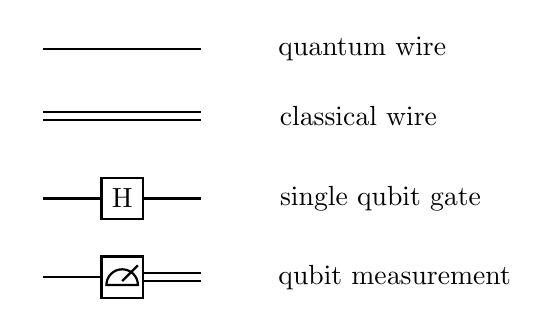
\begin{tikzpicture}[thick]
			
			\tikzstyle{operator} = [draw,fill=white,minimum size=1.5em] 
			
			%\draw (3,3) -- (3,0) ;
			
			\draw (0,3) -- (2,3) ;
			\node at (4.05,3) {quantum wire};
			
			\draw (0,2.1) -- (2,2.1) ;
			\draw (0,2.2) -- (2,2.2) ;
			\node at (4,2.15) {classical wire};
			
			\draw (0,1.1) -- (2,1.1) ;
			\node[operator] (op11) at (1,1.1) {H};
			\node at (4.28,1.1) {single qubit gate};
			
			\draw (0,0.1) -- (1,0.1) ;
			
			\draw (1,0.15) -- (2,0.15) ;
			\draw (1,0.05) -- (2,0.05) ;
			% Define coordinates
			\def\Radius{0.2}
			\path
			(-\Radius, 0) coordinate (A)
			-- coordinate (M)
			(\Radius, 0) coordinate (B)
			(M) +(60:\Radius) coordinate (C)
			+(120:\Radius) coordinate (D)
			;
			
			\node[operator] (op11) at (1,0.1) {};
			\node at (4.46,0.1) {qubit measurement};
			
			% Draw semicircle
			\draw[operator]
			(1.2,0) arc(0:180:\Radius) -- cycle ;
			% Annotations
			
			\draw (1,0.05) -- (1.2,0.25);
			
		\end{tikzpicture}
\end{center}
	
	\subsection{Controlled Gates}
	
	A controlled gate operates on two or more qubits, where one or more qubits act as the "control" qubits, and the others as the "target" qubits. For the context of this thesis, we will discuss controlled operations involving a single control qubit.
	
	Below, we present the quantum circuit and matrix representation of the controlled-X gate, along with its effect on all 2-qubit states:
	
	\begin{figure}[!h]
		\centering
		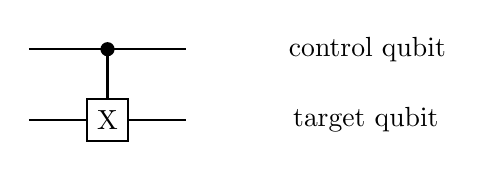
\begin{tikzpicture}[thick]
			
			\tikzstyle{operator} = [draw,fill=white,minimum size=1.5em] 
			
			\draw (0,2) -- (2,2) ;
			\node at (4.30,2) {control qubit};
			
			\draw[black,fill=black] (1,2) circle (.5ex);
			\draw (1, 1.1) -- (1, 2);
			
			\draw (0,1.1) -- (2,1.1) ;
			\node[operator] (op11) at (1,1.1) {X};
			\node at (4.28,1.1) {target qubit};
		\end{tikzpicture}
	\end{figure}	

	
	\begin{align*}	
		CX &= 	\begin{bmatrix}
			\mathbb{I}_2 & 0 \\
			0 & X \\
		\end{bmatrix}= \begin{bmatrix}
		1 & 0 & 0 & 0  \\
		0 &1 & 0 &0 \\
		0 &0 & 0 & 1 \\
		0 &0 & 1 & 0 \\
		\end{bmatrix}
	\end{align*}
	
	\begin{align*}	
		X|00\rangle &= |00\rangle\\
		X|01\rangle &= |01\rangle\\
		X|10\rangle &= |11\rangle\\
		X|11\rangle &= |10\rangle
	\end{align*}
	
	In this operation, only the states $|10\rangle$ and $|11\rangle$ undergo any change. The first qubit, positioned on the left, acts as the control qubit, which determines whether the operation is applied. The second qubit, positioned on the right, is the target qubit and is affected only if the control qubit is in the state $|1\rangle$.
	
	Let us now explore the controlled-Z gate. We will examine the quantum circuit and matrix representation, as well as its effect on all 2-qubit states.
	
	
		\begin{figure}[!h]
		\centering
		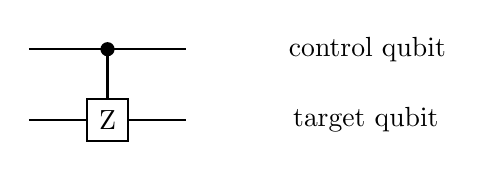
\begin{tikzpicture}[thick]
			
			\tikzstyle{operator} = [draw,fill=white,minimum size=1.5em] 
			
			%\draw (3,3) -- (3,0) ;
			
			\draw (0,2) -- (2,2) ;
			\node at (4.30,2) {control qubit};
			
			\draw[black,fill=black] (1,2) circle (.5ex);
			\draw (1, 1.1) -- (1, 2);
			
			\draw (0,1.1) -- (2,1.1) ;
			\node[operator] (op11) at (1,1.1) {Z};
			\node at (4.28,1.1) {target qubit};
		\end{tikzpicture}
	\end{figure}	
	
	
	\begin{align*}	
		CZ &= 	\begin{bmatrix}
			\mathbb{I}_2 & 0 \\
			0 & Z \\
		\end{bmatrix}= \begin{bmatrix}
			1 & 0 & 0 & 0  \\
			0 &1 & 0 &0 \\
			0 &0 & 1 & 0 \\
			0 &0 & 0 & -1 \\
		\end{bmatrix}
	\end{align*}
	
	\begin{align*}	
		Z|00\rangle &= |00\rangle\\
		Z|01\rangle &= |01\rangle\\
		Z|10\rangle &= |10\rangle\\
		Z|11\rangle &= -|11\rangle
	\end{align*}
	
	In this case, only the final state, $|11\rangle$ was affected, specifically altering the state's phase. We can construct customized controlled gates using any unitary matrix $U$. A controlled-$U$ gate, designed to act on $n$ target qubits, can be represented using block matrix notation. In this context, $\mathbb{I}_n$ denotes the identity matrix which contains $2^{n}$ diagonal elements:
	
		\begin{figure}[!h]
		\centering
		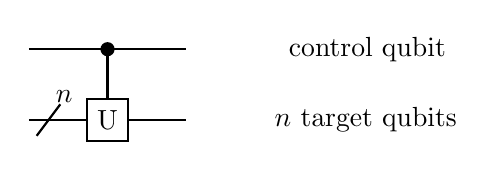
\begin{tikzpicture}[thick]
			
			\tikzstyle{operator} = [draw,fill=white,minimum size=1.5em] 
			
			%\draw (3,3) -- (3,0) ;
			
			\draw (0,2) -- (2,2) ;
			\node at (4.30,2) {control qubit};
			
			\draw[black,fill=black] (1,2) circle (.5ex);
			\draw (1, 1.1) -- (1, 2);
			
			\draw (0,1.1) -- (2,1.1) ;
			\node[operator] (op11) at (1,1.1) {U};
			\node at (4.28,1.1) {$n$ target qubits};
			
			\draw (0.1,0.9) -- (0.4,1.3) ;
			\node at (0.45,1.4) {$n$};
		\end{tikzpicture}
	\end{figure}	
	
	
	\begin{equation}\label{control-u-matrix}
	CU = \begin{bmatrix}
		\mathbb{I}_n & 0 \\
		0 & U \\
	\end{bmatrix}
	\end{equation}

	
	\section{Quantum Phase Estimation}
			The phase estimation algorithm initially proposed by Alexey Kitaev \cite{kitaev1995quantum} plays an important role as a subroutine for the more widely known factoring algorithm by Peter Shor \cite{Shor}. We first must briefly discuss the Quantum Fourier Transform (QFT) as it is key to understanding phase estimation \cite{nielsen00}. Given a computational basis state $|x\rangle$, applying the QFT ($F_N$) results in:
	
	$$ F_N |x \rangle = \frac{1}{\sqrt{N}} \sum_{k=0}^{N-1} e^{2\pi i x k N^{-1}} |k\rangle $$
	
	Let us represent this in binary notation and decompose it into a tensor product. We can represent $|x\rangle$ as a string of bits, and the QFT as a tensor product of single qubit basis states:
	
	$$|x\rangle = |x_1x_2 ... x_n\rangle =  |x_1\rangle \otimes |x_2\rangle \otimes ... \otimes |x_n\rangle$$
	
	\begin{eqnarray}\label{phase-equation}
		F_N |x \rangle = \frac{1}{\sqrt{2^n}} \bigotimes_{j=1}^n (|0\rangle +  e^{2\pi i x  2^{-j}} |1\rangle)
	\end{eqnarray}
	
	$$= \frac{1}{\sqrt{2^n}} ((|0\rangle + \omega_1|1\rangle)  \otimes(|0\rangle + \omega_2|1\rangle)\otimes ... \otimes(|0\rangle + \omega_n|1\rangle))$$
	
	
	\begin{eqnarray*}
		\omega_1 &=& e^{2\pi i x 2^{-1}} =  e^{2\pi i (0.x_n)}\\
		\omega_2 &=& e^{2\pi i x 2^{-2}} =  e^{2\pi i (0.x_{n-1}x_n)}\\
		...\\
		\omega_n &=& e^{2\pi i x 2^{-n}} =  e^{2\pi i (0.x_1...x_n)}
	\end{eqnarray*}
	
	
	An important characteristic of the $w_j$ is the bit shift occurring in the exponent. If we look at $w_1$, the exponent has a factor $x 2^{-1}$, which is equivalent to one right bit shift: $x_1...x_{n-1}.x_n$. Integer multiples of the exponent would imply full rotations returning to the same point. Thus we can ignore all the values on the left of the decimal and what remains is $0.x_n$. 
	
	
	
	Let us discuss the phase estimation problem. Given an eigenstate $|\lambda \rangle$ of a unitary operator $U$, we want to calculate a good approximation  for $\phi \in [0,1)$ satisfying:
	
	\begin{equation}
		U |\lambda \rangle = e^{2\pi i \phi} |\lambda \rangle
	\end{equation}
	
	The phase estimation algorithm uses two registers of qubits. The first one will be a set of $n$ control qubits that determine the precision of our approximation. The second register will be a set of $m$ qubits initialized to an eigenstate $|\lambda\rangle$.
	
	
	\begin{figure}[!h]
		\centering
		\includegraphics[trim={1cm 12cm 11cm 0},clip, width=0.8 \linewidth]{"graphics/phase_circ"}
		\caption{A quantum circuit representation of the phase estimation algorithm. Given $ U |\lambda \rangle = e^{2\pi i \phi} |\lambda \rangle $, this algorithm allows us to generate an  approximation for $\phi \in [0,1)$ . The circuit consists of two registers of qubits. The first $n$-qubits are initialized to $|0\rangle$ and contribute to the precision of the $\phi$ value obtained. The second register of $m$-qubits is initialized to the eigenstate of $U$.  The Hadamard gates, $H$, are used to create a uniform superposition in the first register. The control gates based on $U$ are responsible for encoding phase to the qubits in the first register. Finally, a $QFT^\dagger$ is performed on the first register to extract the encoded phase. Each subsequent qubit in the first register would require double the control gates. Thus, with a large $n$ we obtain a more precise value for $\phi$, but also exponentially increase our computation time.}
		\label{fig:phasrcircuit}
	\end{figure}
	
	
	Let us walk through the quantum circuit in Fig. \ref{fig:phasrcircuit}, to understand the inner workings of this algorithm.	 Our initialized state is $|0^{\otimes n} \lambda\rangle$. From here we perform the same operation we find in (1), where all the qubits in the first register are set to a uniform superposition on all states $2^n$. The next portion of the algorithm involves applying controlled gates based on the unitary operator $U$. The function of these $CU$ gates is to apply the operator $U$ on $|\lambda\rangle$ if the control qubit is in the state $|1\rangle$. We can have a look at the effect on the n\textsuperscript{th} qubit, after it has been prepared in a superposition by the Hadamard gate:
	
	$$ \frac{1}{\sqrt{2}}(|0\rangle + |1\rangle) \otimes |\lambda\rangle =  \frac{1}{\sqrt{2}}(|0 \lambda \rangle + |1 \lambda\rangle)$$
	
	Applying $CU$ and factoring out the eigenstate:
	
	\begin{eqnarray*}
		CU \frac{1}{\sqrt{2}}(|0 \lambda \rangle + |1 \lambda\rangle) &=&  \frac{1}{\sqrt{2}}(CU|0 \lambda \rangle + CU|1 \lambda\rangle )\\
		&=& \frac{1}{\sqrt{2}}(|0 \lambda \rangle + e^{2\pi i \phi}|1 \lambda\rangle)\\
		&=&\frac{1}{\sqrt{2}}( |0 \rangle + e^{2\pi i \phi}|1 \rangle)\otimes |\lambda\rangle
	\end{eqnarray*}
	
	We can see that the eigenstate after the $CU$ operation is left unchanged. The phase has been encoded into the control qubit instead, a result that is due to the phase kickback. Thus, we can reuse our eigenstate for the next qubit. Consecutive qubits have double the number of $CU$ operators as the previous, thus squaring the eigenvalue each time:
	
	\begin{eqnarray*}
		\text{qubit\textsubscript{n-1}} &:&   |0 \rangle + e^{2\pi i \phi 2}|1 \rangle \\
		...\\
		\text{qubit\textsubscript{1}} &:&   |0 \rangle + e^{2\pi i \phi 2^n}|1 \rangle
	\end{eqnarray*}
	
	We know that the value of $\phi < 1$. We can represent this in binary notation in the form $0.\phi_1\phi_2...\phi_n$:
	
	$$\phi = \sum_{j=1}^n \phi_j 2^{-j}$$
	
	If we have another look at the control qubits using binary notation for $\phi$ instead, we can see the result of the multiple $CU$ operations simply results in right bit shifts:
	
	
	\begin{eqnarray*}
		\text{qubit\textsubscript{n}} &:&   |0 \rangle +e^{2\pi i (0.\phi_1\phi_2...\phi_n)}|1 \rangle  \\
		\text{qubit\textsubscript{n-1}} &:&   |0 \rangle + e^{2\pi i (0.\phi_2...\phi_n)}|1 \rangle \\
		...\\
		\text{qubit\textsubscript{1}} &:&   |0 \rangle + e^{2\pi i (0.\phi_n)}|1 \rangle
	\end{eqnarray*}
	
	 After all the $CU$ operations, we look at the form of the first register in the state $|\alpha\rangle$ and it will resemble the result of performing the QFT we saw in Equation \eqref{phase-equation}. Here, our $\omega_j$ are:
	
	\begin{eqnarray*}
		\omega_1 &=& e^{2\pi i x 2^{-1}} =  e^{2\pi i (0.\phi_n)}\\
		\omega_2 &=& e^{2\pi i x 2^{-2}} =  e^{2\pi i (0.\phi_{n-1}\phi_n)}\\
		...\\
		\omega_n &=& e^{2\pi i x 2^{-n}} =  e^{2\pi i (0.\phi_1...\phi_n)}
	\end{eqnarray*}
	Simply performing the inverse QFT will give us $|\phi\rangle =  |\phi_1\phi_2 ... \phi_n\rangle$.  We can immediately see the approximation is limited by the number of qubits in the first register. A simple strategy would be to increase the number of qubits; however this would also increase the computational cost as we double our use of $CU$ gates for each additional qubit.
	
	It is possible that $\phi$ is not a discrete value that can be exactly represented by $n$ qubits, i.e., $|\phi\rangle \neq |\phi_1\phi_2 ... \phi_n\rangle$. Fortunately, this algorithm still provides a good approximation, with the best outcome occurring with a probability of at least $4/{\pi^2} \approx 40\%$. Should the approximation deviate by more than $2^{-n}$, the probability of measuring this less favorable outcome is at most $25\%$ \cite{Phase-estimation}. This concept is further illustrated in Fig. \ref{fig:phase-precision}.
	
\begin{figure}[ht]
	\centering
	% Adjust each subfigure to span full linewidth for vertical stacking
	\begin{subfigure}[b]{\linewidth}
		\centering
		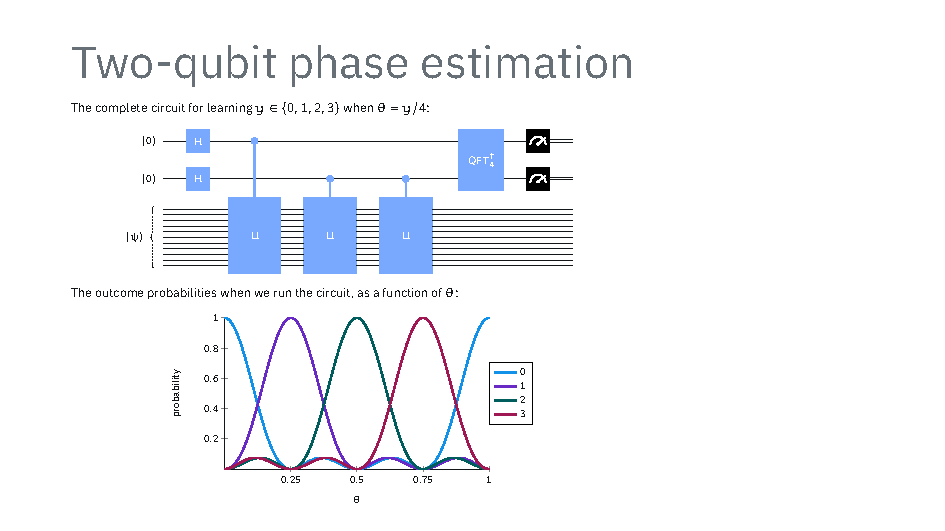
\includegraphics[height=4.5cm, trim={2.9cm 0.4cm 6.9cm 5.2cm}, clip]{phase-lecture/18_Phase-estimation-lecture-slides}
		\caption{2-qubit estimation}
		\label{fig:image1}
	\end{subfigure}
	
	% Add some vertical spacing between subfigures if desired
	\vspace{1ex} % Adjust the space as needed
	
	\begin{subfigure}[b]{\linewidth}
		\centering
		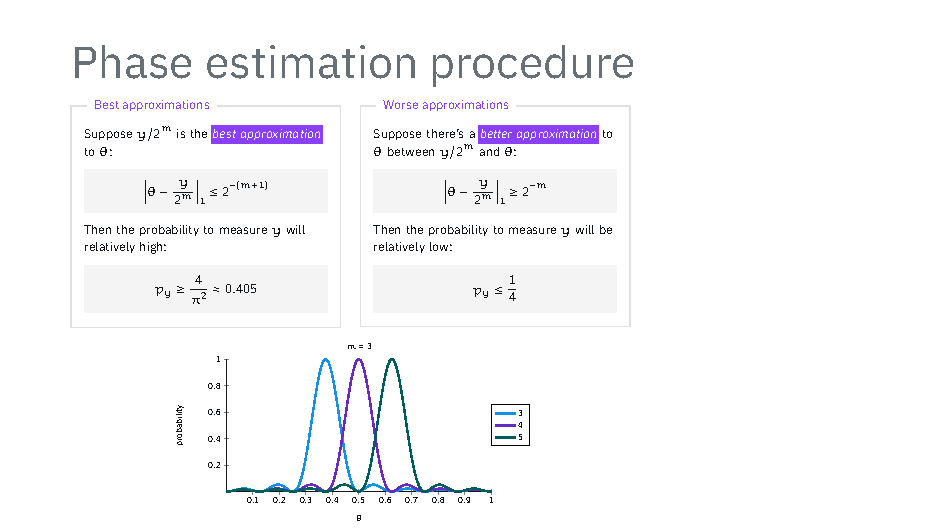
\includegraphics[height=4.5cm, trim={2.9cm 0.15cm 6.9cm 5.95cm}, clip]{phase-lecture/27_Phase-estimation-lecture-slides}
		\caption{3-qubit estimation}
		\label{fig:image2}
	\end{subfigure}
	
	\vspace{1ex} % Adjust the space as needed
	
	\begin{subfigure}[b]{\linewidth}
		\centering
		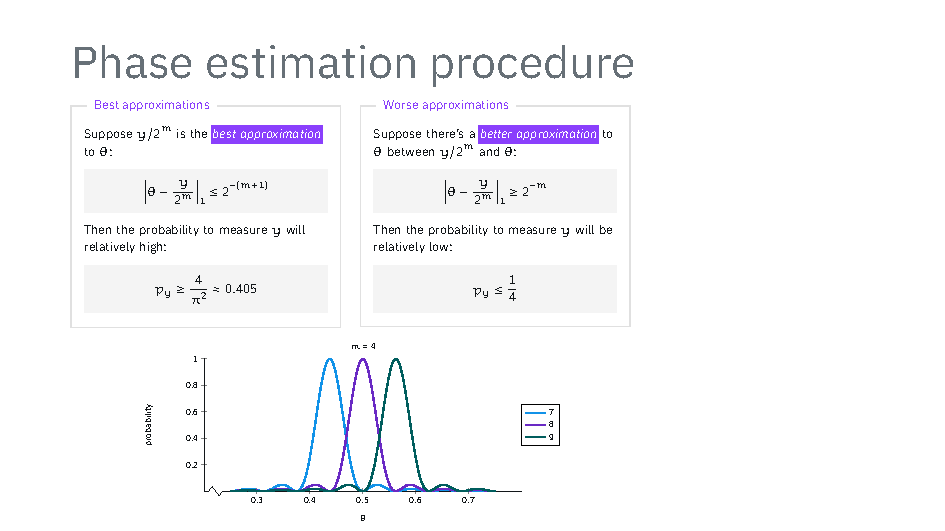
\includegraphics[height=4.5cm, trim={2.4cm 0.15cm 6.4cm 5.95cm}, clip]{phase-lecture/28_Phase-estimation-lecture-slides}
		\caption{4-qubit estimation}
		\label{fig:image3}
	\end{subfigure}
	
	\vspace{1ex} % Adjust the space as needed
	
	\begin{subfigure}[b]{\linewidth}
		\centering
		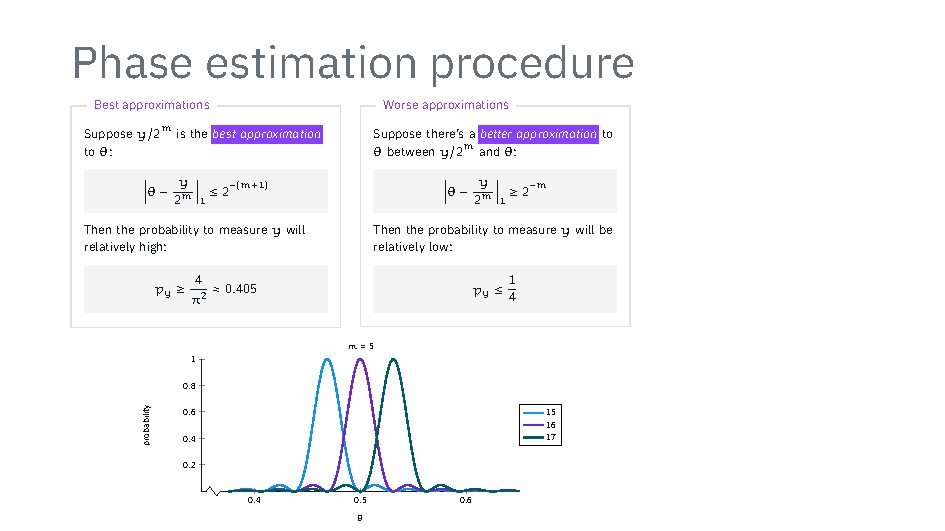
\includegraphics[height=4.5cm, trim={2.4cm 0.15cm 6.4cm 5.95cm}, clip]{phase-lecture/29_Phase-estimation-lecture-slides}
		\caption{5-qubit estimation}
		\label{fig:image4}
	\end{subfigure}
	
	\caption{Varying degree of precision by the phase estimation algorithm as a function of the number of qubits (2, 3, 4, and 5). \cite{Phase-estimation}.}
	\label{fig:phase-precision}
\end{figure}
	
	%A simple example of minimizing the bottleneck travelling salesman problem (maybe with images):
	%an example of storing phases and using phase estimation
	%grover's search explanation
	\chapter{Algorithm}
	
The decision problem of the BTSP seeks to determine if there exists a Hamiltonian cycle where the weight of each edge is less than a specified threshold $\alpha$. In such a cycle, if we denote the weight of any edge as $\gamma_i$, then it must satisfy the condition:
	
	\begin{equation}\label{constraint-alpha} 
	 \gamma_i < \alpha
	\end{equation}
	
	We will construct the algorithm in the following steps:
	\begin{enumerate}
		\item Normalize edge weights to ensure that no single Hamiltonian cycle's total weight is greater than or equal to 1, allowing for effective use of the phase estimation algorithm.\\
		\item Construct a unitary operator that encodes information about the Hamiltonian cycles, representing these as phases along its diagonal. Our approach aligns with the findings presented by Ramakrishnan, Sharma, and Punnen \cite{srinivasan2018efficient}.\\
		\item Set all edge weights $\geq \alpha$ to zero and construct a secondary unitary operator similar to the one described in Step 2.\\
		\item Create controlled gates using the unitary operators constructed in Step 2 and 3.\\
		\item Identify all the eigenstates of the unitary operators that map to the phases associated with the Hamiltonian cycles.\\
		\item Perform phase estimation twice, using the same eigenstate and controlled gates, to evaluate the Hamiltonian cycle both before and after setting edge weights $\geq \alpha$ to zero.\\
		\item Compare the two resulting phases; if they match, the Hamiltonian cycle under examination satisfies the condition and is a viable solution.\\
		
	\end{enumerate}
		
	\section{Normalize Edge Weights}
	
		A Hamiltonian cycle of a complete graph with $N$ nodes requires $N$ edge weights to complete the cycle. A single graph consists of a total of $N(N-1)$ edge weights in a directed graph. We can choose the largest $N$ and use these to normalize the edge weights. Let $w$ represent our edge-weights, which will be a list of $m = N(N-1)$ elements:
	
	$$w = \{w_1, w_2, \ldots, w_m\}$$ 
	
	Sort $w$ in descending order to obtain:
	
	\begin{equation}\label{sorted-weights}
	w' = \{w'_1, w'_2, \ldots, w'_m\}
	\end{equation}
	
	Where: \begin{itemize}
		\item[] $w'_1 \geq w'_2 \geq \ldots \geq w'_m$
		\end{itemize}
		
The sum $S$ of the largest $N$ items in $w$ can be described as:

\begin{equation}\label{sum-S}
S = \sum_{i=1}^{N} w'_i
\end{equation}

  We can now perform the normalization. Let $\tilde{w}$ describe our normalized edge-weights:
  
 \begin{equation}\label{normalization}
  	\tilde{w} = (S + \epsilon)^{-1}w
\end{equation}

Where: \begin{itemize}
	\item[] $\epsilon > 0$
\end{itemize}
The purpose of $\epsilon$ is to ensure that if any normalized Hamiltonian cycle's weight is exactly equal to $S$, it does not result in a zero phase.
	
	
	\section{Unitary Operator and Eigenstates associated with the Hamiltonian Cycles}
	
	We begin by constructing diagonal matrices $U_j$, one for each node in a complete graph, and describing the elements of these matrices:
	
	\begin{equation}\label{Uj-elements}
	\left[U_j \right]_{kk} = e^{2\pi i\gamma_{jk} (1 - \delta_{jk})}
	\end{equation}
	
	Where:	\begin{itemize}
		\item[]  $ 1 \leq j, k \leq N$
		\item[]  $N$ denotes the total number of nodes.
		\item[]  $\gamma_{jk}$ represents the edgeweight connecting node $j\rightarrow k$.
	\end{itemize}
	
	
	Next, we construct $U$, which is the tensor product of all the diagonal matrices:
	\begin{equation}\label{U-tensor}
	 U = \bigotimes_j^N U_j
	 \end{equation}
	
	
	$U$ will be a $N^N \times N^N$ matrix with only the diagonal elements populated. Because the diagonal elements consist entirely of phases, $\left[U \right]_{kk} = e^{i\alpha_{kk}} $, we can confirm the unitary operator condition, $U^\dagger U = \mathds{1}$, is satisfied.
	
	
	Given $U$'s diagonal nature, its eigenstates align with the basis computational states. We specifically focus on eigenstates that correspond to Hamiltonian cycles, which are determined by their phases. To understand how the diagonal elements of $U$ are derived from the individual $U_j$ matrices, we examine the tensor product construction. This process fills the diagonal elements of $U$, thus simplifying our approach by allowing us to directly consider these elements.
	
	\begin{flalign*}
	[U]_{0} & = [U_1]_{0}\cdot [U_2] _{0}\cdot \ldots  \cdot [U_{N-2}]_{0} \cdot [U_{N-1}]_{0}\cdot [U_N]_{0} \\
	[U]_{1}  & = [U_1]_{0}\cdot [U_2] _{0}\cdot \ldots \cdot [U_{N-2}]_{0}\cdot [U_{N-1}]_{0}\cdot [U_N]_{1}\\
	&  \vdots\\
	[U]_{N-1} &= [U_1]_{0}\cdot [U_2] _{0}\cdot \ldots\cdot [U_{N-2}]_{0} \cdot [U_{N-1}]_{0}\cdot [U_N]_{N-1}\\
	[U]_{N} &= [U_1]_{0}\cdot [U_2] _{0}\cdot \ldots \cdot [U_{N-2}]_{0} \cdot [U_{N-1}]_{1}\cdot [U_N]_{0}\\
	& \vdots\\
	[U]_{2N - 1} & = [U_1]_{0}\cdot [U_2] _{0}\cdot \ldots \cdot [U_{N-2}]_{0} \cdot [U_{N-1}]_{1}\cdot [U_N]_{N-1}\\
	[U]_{2N} &= [U_1]_{0}\cdot [U_2] _{0}\cdot \ldots \cdot [U_{N-2}]_{0} \cdot [U_{N-1}]_{2}\cdot [U_N]_{0}\\
	& \vdots\\
	[U]_{N^2 - 1 } & = [U_1]_{0}\cdot [U_2] _{0}\cdot \ldots \cdot [U_{N-2}]_{0} \cdot [U_{0}]_{N-1}\cdot [U_N]_{N-1}\\
	[U]_{N^2} &= [U_1]_{0}\cdot [U_2] _{0}\cdot \ldots \cdot [U_{N-2}]_{1} \cdot [U_{N-1}]_{0}\cdot [U_N]_{0}\\
	& \vdots\\
	[U]_{N^2 + N - 1} & = [U_1]_{0}\cdot [U_2] _{0}\cdot \ldots \cdot [U_{N-2}]_{1} \cdot [U_{N-1}]_{0}\cdot [U_N]_{N-1}\\
	[U]_{N^2 + N } &= [U_1]_{0}\cdot [U_2] _{0}\cdot \ldots \cdot [U_{N-2}]_{1} \cdot [U_{N-1}]_{1}\cdot [U_N]_{0}\\
	&  \vdots\\
	[U]_{N^3- 1} & = [U_1]_{0}\cdot [U_2] _{0}\cdot \ldots \cdot [U_{N-2}]_{N-1} \cdot [U_{N-1}]_{N-1}\cdot [U_N]_{N-1}
	\end{flalign*}
	This pattern indicates:
	\begin{equation}\label{U-matrix-eq}
	[U]_{k} = [U_1]_{\alpha_{N-1}}\cdot [U_2] _{\alpha_{N-2}}\cdot \ldots \cdot [U_{N-2}]_{\alpha_2} \cdot [U_{2}]_{\alpha_{1}}\cdot [U_N]_{\alpha_{0}}
	\end{equation}
	
	Where: \begin{itemize}
		\item[] $\alpha_i = \left(k//\left(N^{i}\right)\right) \% N$
		\item[] $//$ denotes integer division
	    \item[] $\%$ is the modulus operation
	    \end{itemize}
	
	
	
	
 	We observe that this pattern follows base-$N$ counting, where $N$ is the total number of nodes. Converting $k$ into base-$N$ yields the indices of our original diagonal matrices. To identify the relevant eigenstates, we first locate the elements in $U_j$ associated with a Hamiltonian cycle. Then, we retrieve their respective indices and convert this sequence from base-$N$ to $k$. This process allows us to identify our eigenstate $|k\rangle$. 
	
	\subsection{The Four City Graph}
	
	
	\begin{center}	
	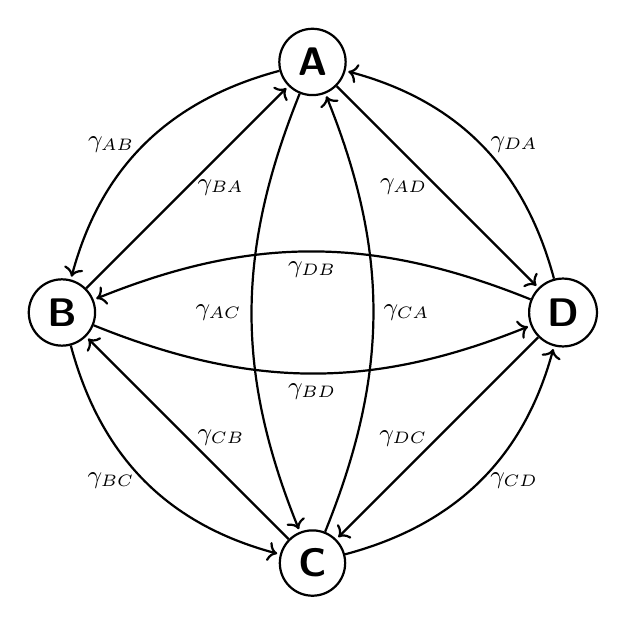
\begin{tikzpicture}[->,shorten >=1pt,auto,node distance=4.5cm, thick,main node/.style={circle,draw,font=\sffamily\Large\bfseries}]
		
		\node[main node] (1) {A};
		\node[main node] (2) [below left of=1] {B};
		\node[main node] (3) [below right of=2] {C};
		\node[main node] (4) [below right of=1] {D};
		
		\path[every node/.style={font=\sffamily\small}]
		(1) edge node [left] {$\gamma_{AD}$} (4)
		edge [bend right] node[left] {$\gamma_{AB}$} (2)
		edge[bend right=22] node[left] {$\gamma_{AC}$} (3)
		%edge [loop above] node {0.1} (1)
		(2) edge node [right] {$\gamma_{BA}$} (1)
		edge[bend right=22] node[below] {$\gamma_{BD}$} (4)
		%edge [loop left] node {0.4} (2)
		edge [bend right] node[left] {$\gamma_{BC}$} (3)
		(3) edge node [right] {$\gamma_{CB}$} (2)
		edge [bend right] node[right] {$\gamma_{CD}$} (4)
		edge[bend right=22] node[right] {$\gamma_{CA}$} (1)
		(4) edge node [left] {$\gamma_{DC}$} (3)
		%edge [loop right] node {0.6} (4)
		edge[bend right=22] node {$\gamma_{DB}$} (2)
		edge [bend right] node[right] {$\gamma_{DA}$} (1);
	\end{tikzpicture}
	
	\end{center}
	
	
	
	For the 4-city graph, we will begin with four matrices to represent the 12 edge weights. Utilizing Equation \eqref{Uj-elements}, where $j, k \in \{A, B, C, D\}$, we can construct matrix $A$:

	$$
	A = \begin{bmatrix}
		1 & 0 & 0 & 0 \\
		0 & e^{i2\pi\gamma_{AB}} & 0 & 0 \\
		0 & 0 & e^{i2\pi\gamma_{AC}} & 0 \\
		0 & 0 & 0 & e^{i2\pi\gamma_{AD}} \\
	\end{bmatrix}
	$$
	
	Since we only populate the diagonal elements, we can ignore the other elements of the matrix. Let $ a = \mathrm{diag}(A)$, and let us construct the other diagonals:
	
	\begin{align*}	
		a & = \begin{bmatrix}
			1 \\
			e^{i2\pi\gamma_{AB}} \\
			e^{i2\pi\gamma_{AC}} \\
			e^{i2\pi\gamma_{AD}} \\
		\end{bmatrix} 
		b  = \begin{bmatrix}
			e^{i2\pi\gamma_{BA}} \\
			1 \\
			e^{i2\pi\gamma_{BC}} \\
			e^{i2\pi\gamma_{BD}} \\
		\end{bmatrix}
		c  = \begin{bmatrix}
			e^{i2\pi\gamma_{CA}} \\
			e^{i2\pi\gamma_{CB}} \\
			1 \\
			e^{i2\pi\gamma_{CD}} \\
		\end{bmatrix} 
		d = \begin{bmatrix}
			e^{i2\pi\gamma_{DA}} \\
			e^{i2\pi\gamma_{DB}} \\
			e^{i2\pi\gamma_{DC}} \\
			1 \\
		\end{bmatrix} 						 			
	\end{align*}
	
	
	Next, we construct the tensor product with Equation \eqref{U-tensor}:
	
	\begin{equation}\label{4-city-matrix-tensor}
	 U = A \otimes B \otimes C \otimes D
	\end{equation}
	
	For the sake of convenience in dealing only with the diagonals, we can similarly state $ u = \mathrm{diag}(U)$, thus:
	
	$$ u = a \otimes b \otimes c \otimes d$$
	
	
	Referring to Equation \eqref{U-matrix-eq} concerning the matrix elements for $U$,  the diagonal elements for the 4-city graph will simplify to:
	
	\begin{equation}\label{4-city-tensor}
		u_{k} = a_{\alpha_{3}}\cdot b _{\alpha_{2}} \cdot c_{\alpha_1} \cdot d_{\alpha_{0}}
	\end{equation}
	
	Where:
	\begin{itemize}
	\item[] $\alpha_i = \left(k//\left(4^{i}\right)\right) \% 4$
	\end{itemize}
	
	Let us proceed with identifying the eigenstate corresponding to a specific Hamiltonian cycle. Let us consider the cycle represented by the following path:
	
	\begin{equation}\label{one-ham-cycle-4-city}
		A \rightarrow D \rightarrow B \rightarrow C \rightarrow A
	\end{equation}
	
	From this point, we can identify the edge weights that are relevant to us:
	
	\begin{equation*}
		\gamma_{AD} + \gamma_{DB} + \gamma_{BC} + \gamma_{CA}
	\end{equation*}
	
	Therefore, the phase we aim to estimate would be determined by the following element product:
	
	\begin{equation*}
		\Large{a_{3} \cdot d_{1} \cdot b_{2} \cdot c_{0} = e^{i2\pi (\gamma_{AD} + \gamma_{DB} + \gamma_{BC} + \gamma_{CA})}}
	\end{equation*}
	
	
	To correctly identify the eigenstate, we need to rearrange the product to match the form of Equation \eqref{4-city-tensor}:
	
	\begin{equation*}
		\Large{a_{3} \cdot d_{1} \cdot b_{2} \cdot c_{0} = \Large{a_{3}} \cdot b_{2} \cdot c_{0}  \cdot d_{1}}
	\end{equation*}
	
	From here, we simply read out the indices. Based on our discussion under Equation \eqref{U-matrix-eq}, we can infer that we are working in base 4. Thus, we simply need to convert to base 10 to understand the exact column number and to base 2 to be used as the initialized eigenstate.
	
	\begin{equation*}
		\text{base } 4 = 3201 \leftrightarrow \text{base } 10 = 225 \leftrightarrow  \text{base } 2 = 11100001
	\end{equation*}
	

Thus, our eigenstate for Hamiltonian cycle \eqref{one-ham-cycle-4-city} will be $|225\rangle$ or $|11100001\rangle$. We can perform an identical process for all the Hamiltonian cycles to find their corresponding eigenstates. These are all listed in Table \ref{table:ham-cycle-details-4-city} and Table \ref{table:4-city-conversions}.
	
	
	\begin{table}[h]
		\centering
		\begin{tabular}{|c|c|c|}
			\hline
			\textbf{Hamiltonian Cycle} & \textbf{Total Cost} & \textbf{Diagonal Elements Product} \\
			\hline
			$A \rightarrow B \rightarrow C \rightarrow D \rightarrow A$ & $\gamma_{AB} + \gamma_{BC} + \gamma_{CD} + \gamma_{DA}$ & $a_{1} \cdot b_{2} \cdot c_{3} \cdot d_{0}$ \\
			$A \rightarrow B \rightarrow D \rightarrow C \rightarrow A$ & $\gamma_{AB} + \gamma_{BD} + \gamma_{DC} + \gamma_{CA}$ & $a_{1} \cdot b_{3} \cdot d_{2} \cdot c_{0}$ \\
			$A \rightarrow C \rightarrow B \rightarrow D \rightarrow A$ & $\gamma_{AC} + \gamma_{CB} + \gamma_{BD} + \gamma_{DA}$ & $a_{2} \cdot c_{1} \cdot b_{3} \cdot d_{0}$ \\
			$A \rightarrow C \rightarrow D \rightarrow B \rightarrow A$ & $\gamma_{AC} + \gamma_{CD} + \gamma_{DB} + \gamma_{BA}$ & $a_{2} \cdot c_{3} \cdot d_{1} \cdot b_{0}$ \\
			$A \rightarrow D \rightarrow B \rightarrow C \rightarrow A$ & $\gamma_{AD} + \gamma_{DB} + \gamma_{BC} + \gamma_{CA}$ & $a_{3} \cdot d_{1} \cdot b_{2} \cdot c_{0}$ \\
			$A \rightarrow D \rightarrow C \rightarrow B \rightarrow A$ & $\gamma_{AD} + \gamma_{DC} + \gamma_{CB} + \gamma_{BA}$ & $a_{3} \cdot d_{2} \cdot c_{1} \cdot b_{0}$ \\
			\hline
			\end{tabular}
					\caption{Hamiltonian cycles of the directed 4-city graph with their total cost and diagonal element products (\ref{4-city-tensor}).}
			\label{table:ham-cycle-details-4-city}
	\end{table}
	\begin{table}[h]
		\centering
		\begin{tabular}{|c|c|c|}	
			
			\hline
			\textbf{Rearranged Indices (Base 4)} & \textbf{Base 10} & \textbf{Base 2} \\
			\hline
			1230 & 108 & 01101100 \\
			1302 & 114 & 01110010 \\
			2310 & 180 & 10110100 \\
			2031 & 141 & 10001101 \\
			3201 & 225 & 11100001 \\
			3012 & 198 & 11000110 \\
			\hline
		\end{tabular}
		\caption{Eigenstates of matrix $U$ (\ref{4-city-matrix-tensor}), containing the total cost of a Hamiltonian cycle after normalization of the directed 4-city graph.}
		\label{table:4-city-conversions}
	\end{table}
	
	\subsection{The Five City Graph}
	
	
	
		\begin{center}	
		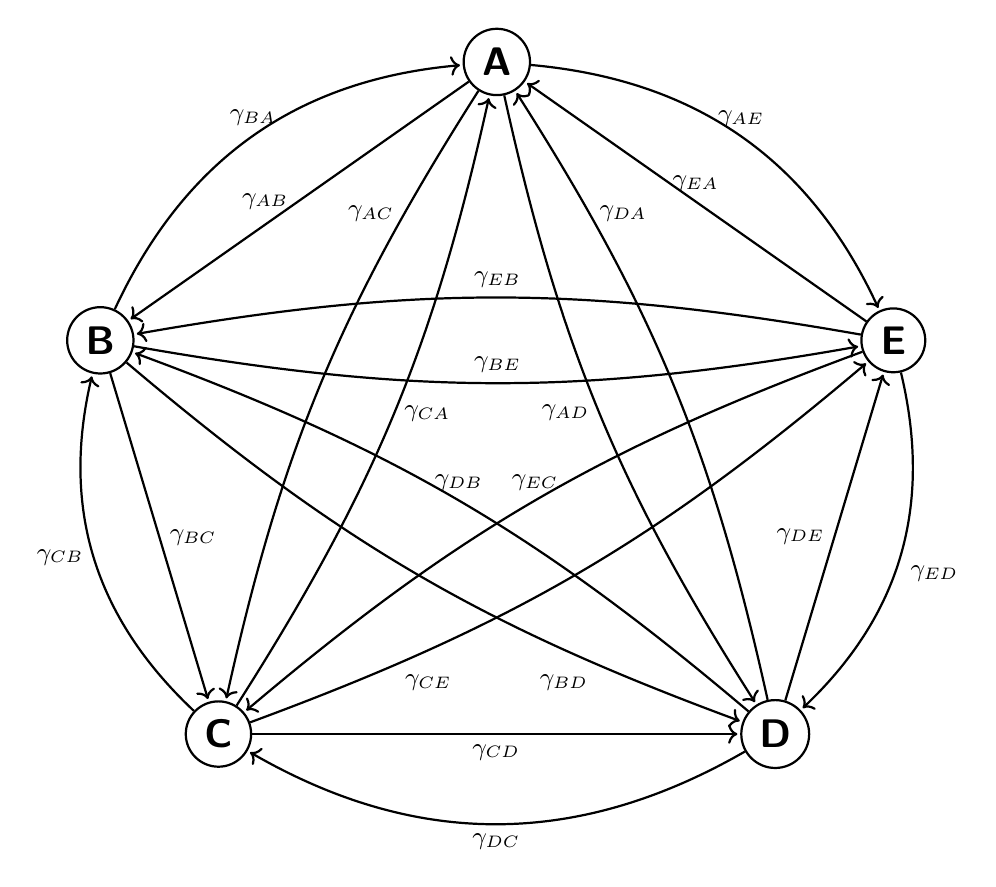
\begin{tikzpicture}[->,shorten >=1pt,auto,node distance=5cm, thick,main node/.style={circle,draw,font=\sffamily\Large\bfseries}]
			
			\node[main node] (1) {A};
			\node[main node] (2) [below left of=1, xshift = -1.5cm] {B};
			\node[main node] (3) [below of=2, xshift= 1.5cm] {C};
			\node[main node] (5) [below right of=1, xshift = 1.5cm] {E};
			\node[main node] (4) [below of=5, xshift= -1.5cm] {D};
			
			\path[every node/.style={font=\sffamily\small}]
			(1) edge [bend right=10] node [left] {$\gamma_{AD}$} (4)
			edge node[left] {$\gamma_{AB}$} (2)
			edge [bend right=10] node[left, pos = 0.2] {$\gamma_{AC}$} (3)
			edge[bend left] node[above] {$\gamma_{AE}$} (5)

			(2) edge[bend left] node [above] {$\gamma_{BA}$} (1)
			edge [bend right=10]  node[below left , pos = 0.8] {$\gamma_{BD}$} (4)
			edge node[right] {$\gamma_{BC}$} (3)
			edge [bend right=10] node[above] {$\gamma_{BE}$} (5)
			
			(3) edge[bend left] node [left] {$\gamma_{CB}$} (2)
			edge node[below] {$\gamma_{CD}$} (4)
			edge [bend right=10] node[right] {$\gamma_{CA}$} (1)
			edge [bend right=10] node[below right , pos = 0.2] {$\gamma_{CE}$} (5)
			
			(4) edge[bend left] node[below] {$\gamma_{DC}$} (3)
			edge [bend right=10] node[above] {$\gamma_{DB}$} (2)
			edge [bend right=10] node[right, pos = 0.8] {$\gamma_{DA}$} (1)
			edge node[left] {$\gamma_{DE}$} (5)
			
			(5) edge node [above] {$\gamma_{EA}$} (1)
			edge [bend right=10]  node[above] {$\gamma_{EB}$} (2)
			edge [bend right=10] node[above] {$\gamma_{EC}$} (3)
			edge[bend left] node {$\gamma_{ED}$} (4);

		\end{tikzpicture}
		
	\end{center}
	
	
		For the 5-city graph, we will begin with five matrices to represent the 20 edge weights. Utilizing Equation \eqref{Uj-elements}, where $j, k \in \{A, B, C, D, E\}$, we can construct matrix $A$:
	
	\begin{equation}\label{5-city-matrix-tensor}
		U = A \otimes B \otimes C \otimes D \otimes E
	\end{equation}
	
	 Similar to the four-city graph, we only populate the diagonal elements. Let  $a=\mathrm{diag}(A)$, and let us construct the other diagonals:
	
	\begin{align*}	
		a & = \begin{bmatrix}
			1 \\
			e^{i2\pi\gamma_{AB}} \\
			e^{i2\pi\gamma_{AC}} \\
			e^{i2\pi\gamma_{AD}} \\
			e^{i2\pi\gamma_{AE}} \\
		\end{bmatrix} 
		b  = \begin{bmatrix}
			e^{i2\pi\gamma_{BA}} \\
			1 \\
			e^{i2\pi\gamma_{BC}} \\
			e^{i2\pi\gamma_{BD}} \\
			e^{i2\pi\gamma_{BE}} \\
		\end{bmatrix}
		c  = \begin{bmatrix}
			e^{i2\pi\gamma_{CA}} \\
			e^{i2\pi\gamma_{CB}} \\
			1 \\
			e^{i2\pi\gamma_{CD}} \\
			e^{i2\pi\gamma_{CE}} \\
		\end{bmatrix} 
		d = \begin{bmatrix}
			e^{i2\pi\gamma_{DA}} \\
			e^{i2\pi\gamma_{DB}} \\
			e^{i2\pi\gamma_{DC}} \\
			1 \\
			e^{i2\pi\gamma_{DE}} \\
		\end{bmatrix}  
		e = \begin{bmatrix}
			e^{i2\pi\gamma_{EA}} \\
			e^{i2\pi\gamma_{EB}} \\
			e^{i2\pi\gamma_{EC}} \\
			e^{i2\pi\gamma_{ED}} \\
			1 \\
		\end{bmatrix}		 			
	\end{align*}
	

	
	We can similarly state $ u = \mathrm{diag}(U)$, thus:
	
	$$ u = a \otimes b \otimes c \otimes d \otimes e$$
	
	
	Referring to Equation \eqref{U-matrix-eq} concerning the matrix elements for U,  the diagonal elements for the 5-city graph will simplify to:
	
	\begin{equation}\label{5-city-tensor}
		u_{k} = a_{\alpha_{4}}\cdot b _{\alpha_{3}} \cdot c_{\alpha_2} \cdot d_{\alpha_{1}}\cdot e_{\alpha_{0}}
	\end{equation}
	
	Where:
	\begin{itemize}
		\item[] $\alpha_i = \left(k//\left(5^{i}\right)\right) \% 5$
	\end{itemize}
	
	
	\vspace{0.5cm}
	
	Let us proceed with identifying the eigenstate corresponding to a specific Hamiltonian cycle. Let us consider the cycle represented by the following path:
	
	\begin{equation}\label{one-ham-cycle-5-city}
		A \rightarrow E \rightarrow D \rightarrow C \rightarrow B \rightarrow A
	\end{equation}
	
	From this point, we can identify the edge weights that are relevant to us:
	
	\begin{equation*}
		\gamma_{AE} + \gamma_{ED} + \gamma_{DC} + \gamma_{CB} + \gamma_{BA}
	\end{equation*}
	
	Therefore, the phase we aim to estimate would be determined by the following element product:
	
	\begin{equation*}
		\Large{a_{4} \cdot e_{3} \cdot d_{2} \cdot c_{1} \cdot b_{0} = e^{i2\pi (\gamma_{AE} + \gamma_{ED} + \gamma_{DC} + \gamma_{CB} + \gamma_{BA})}}
	\end{equation*}
	
	
	To correctly identify the eigenstate, we need to rearrange the product to match the form of Equation \eqref{5-city-tensor}:
	
	\begin{equation*}
		\Large{a_{4} \cdot e_{3} \cdot d_{2} \cdot c_{1} \cdot b_{0}= a_{4} \cdot b_{0}  \cdot c_{1}\cdot d_{2} \cdot e_{3}}
	\end{equation*}
	
	From here, we simply read out the indices. Based on our discussion under Equation \eqref{U-matrix-eq}, we can infer that we are working in base 5. Thus, we simply need to convert to base 10 to understand the exact column number and to base 2 to be used as the initialized eigenstate.
	
	\begin{equation*}
		\text{base } 5 = 40123 \leftrightarrow \text{base } 10 = 2538 \leftrightarrow  \text{base } 2 = 100111101010
	\end{equation*}
	
	Thus, our eigenstate for Hamiltonian cycle \eqref{one-ham-cycle-5-city} will be $|2538\rangle$ or $|100111101010\rangle$. We can perform an identical process for all the Hamiltonian cycles to find their corresponding eigenstates. These are all listed in Table \ref{table:ham-cycle-details-5-city} and Table \ref{table:5-city-conversions}.
	
	
	
	
	\begin{table}[h]
		\centering
		\begin{tabular}{|c|c|c|}
			\hline
			\textbf{Hamiltonian Cycle} & \textbf{Total Cost} & \textbf{Matrix Elements Product} \\
			\hline
$A \rightarrow B \rightarrow C \rightarrow D \rightarrow E \rightarrow A$ & $ \gamma_{AB} + \gamma_{BC} + \gamma_{CD} + \gamma_{DE} + \gamma_{EA}$ & $a_1  \cdot b_2 \cdot c_3 \cdot d_4 \cdot e_0$ \\
$A \rightarrow B \rightarrow C \rightarrow E \rightarrow D \rightarrow A$ & $ \gamma_{AB} + \gamma_{BC} + \gamma_{CE} + \gamma_{ED} + \gamma_{DA}$ & $a_1  \cdot b_2 \cdot c_4 \cdot e_3 \cdot d_0$ \\
$A \rightarrow B \rightarrow D \rightarrow C \rightarrow E \rightarrow A$ & $ \gamma_{AB} + \gamma_{BD} + \gamma_{DC} + \gamma_{CE} + \gamma_{EA}$ & $a_1  \cdot b_3 \cdot d_2 \cdot c_4 \cdot e_0$ \\
$A \rightarrow B \rightarrow D \rightarrow E \rightarrow C \rightarrow A$ & $ \gamma_{AB} + \gamma_{BD} + \gamma_{DE} + \gamma_{EC} + \gamma_{CA}$ & $a_1  \cdot b_3 \cdot d_4 \cdot e_2 \cdot c_0$ \\
$A \rightarrow B \rightarrow E \rightarrow C \rightarrow D \rightarrow A$ & $ \gamma_{AB} + \gamma_{BE} + \gamma_{EC} + \gamma_{CD} + \gamma_{DA}$ & $a_1  \cdot b_4 \cdot e_2 \cdot c_3 \cdot d_0$ \\
$A \rightarrow B \rightarrow E \rightarrow D \rightarrow C \rightarrow A$ & $ \gamma_{AB} + \gamma_{BE} + \gamma_{ED} + \gamma_{DC} + \gamma_{CA}$ & $a_1  \cdot b_4 \cdot e_3 \cdot d_2 \cdot c_0$ \\
$A \rightarrow C \rightarrow B \rightarrow D \rightarrow E \rightarrow A$ & $ \gamma_{AC} + \gamma_{CB} + \gamma_{BD} + \gamma_{DE} + \gamma_{EA}$ & $a_2  \cdot c_1 \cdot b_3 \cdot d_4 \cdot e_0$ \\
$A \rightarrow C \rightarrow B \rightarrow E \rightarrow D \rightarrow A$ & $ \gamma_{AC} + \gamma_{CB} + \gamma_{BE} + \gamma_{ED} + \gamma_{DA}$ & $a_2  \cdot c_1 \cdot b_4 \cdot e_3 \cdot d_0$ \\
$A \rightarrow C \rightarrow D \rightarrow B \rightarrow E \rightarrow A$ & $ \gamma_{AC} + \gamma_{CD} + \gamma_{DB} + \gamma_{BE} + \gamma_{EA}$ & $a_2  \cdot c_3 \cdot d_1 \cdot b_4 \cdot e_0$ \\
$A \rightarrow C \rightarrow D \rightarrow E \rightarrow B \rightarrow A$ & $ \gamma_{AC} + \gamma_{CD} + \gamma_{DE} + \gamma_{EB} + \gamma_{BA}$ & $a_2  \cdot c_3 \cdot d_4 \cdot e_1 \cdot b_0$ \\
$A \rightarrow C \rightarrow E \rightarrow B \rightarrow D \rightarrow A$ & $ \gamma_{AC} + \gamma_{CE} + \gamma_{EB} + \gamma_{BD} + \gamma_{DA}$ & $a_2  \cdot c_4 \cdot e_1 \cdot b_3 \cdot d_0$ \\
$A \rightarrow C \rightarrow E \rightarrow D \rightarrow B \rightarrow A$ & $ \gamma_{AC} + \gamma_{CE} + \gamma_{ED} + \gamma_{DB} + \gamma_{BA}$ & $a_2  \cdot c_4 \cdot e_3 \cdot d_1 \cdot b_0$ \\
$A \rightarrow D \rightarrow B \rightarrow C \rightarrow E \rightarrow A$ & $ \gamma_{AD} + \gamma_{DB} + \gamma_{BC} + \gamma_{CE} + \gamma_{EA}$ & $a_3  \cdot d_1 \cdot b_2 \cdot c_4 \cdot e_0$ \\
$A \rightarrow D \rightarrow B \rightarrow E \rightarrow C \rightarrow A$ & $ \gamma_{AD} + \gamma_{DB} + \gamma_{BE} + \gamma_{EC} + \gamma_{CA}$ & $a_3  \cdot d_1 \cdot b_4 \cdot e_2 \cdot c_0$ \\
$A \rightarrow D \rightarrow C \rightarrow B \rightarrow E \rightarrow A$ & $ \gamma_{AD} + \gamma_{DC} + \gamma_{CB} + \gamma_{BE} + \gamma_{EA}$ & $a_3  \cdot d_2 \cdot c_1 \cdot b_4 \cdot e_0$ \\
$A \rightarrow D \rightarrow C \rightarrow E \rightarrow B \rightarrow A$ & $ \gamma_{AD} + \gamma_{DC} + \gamma_{CE} + \gamma_{EB} + \gamma_{BA}$ & $a_3  \cdot d_2 \cdot c_4 \cdot e_1 \cdot b_0$ \\
$A \rightarrow D \rightarrow E \rightarrow B \rightarrow C \rightarrow A$ & $ \gamma_{AD} + \gamma_{DE} + \gamma_{EB} + \gamma_{BC} + \gamma_{CA}$ & $a_3  \cdot d_4 \cdot e_1 \cdot b_2 \cdot c_0$ \\
$A \rightarrow D \rightarrow E \rightarrow C \rightarrow B \rightarrow A$ & $ \gamma_{AD} + \gamma_{DE} + \gamma_{EC} + \gamma_{CB} + \gamma_{BA}$ & $a_3  \cdot d_4 \cdot e_2 \cdot c_1 \cdot b_0$ \\
$A \rightarrow E \rightarrow B \rightarrow C \rightarrow D \rightarrow A$ & $ \gamma_{AE} + \gamma_{EB} + \gamma_{BC} + \gamma_{CD} + \gamma_{DA}$ & $a_4  \cdot e_1 \cdot b_2 \cdot c_3 \cdot d_0$ \\
$A \rightarrow E \rightarrow B \rightarrow D \rightarrow C \rightarrow A$ & $ \gamma_{AE} + \gamma_{EB} + \gamma_{BD} + \gamma_{DC} + \gamma_{CA}$ & $a_4  \cdot e_1 \cdot b_3 \cdot d_2 \cdot c_0$ \\
$A \rightarrow E \rightarrow C \rightarrow B \rightarrow D \rightarrow A$ & $ \gamma_{AE} + \gamma_{EC} + \gamma_{CB} + \gamma_{BD} + \gamma_{DA}$ & $a_4  \cdot e_2 \cdot c_1 \cdot b_3 \cdot d_0$ \\
$A \rightarrow E \rightarrow C \rightarrow D \rightarrow B \rightarrow A$ & $ \gamma_{AE} + \gamma_{EC} + \gamma_{CD} + \gamma_{DB} + \gamma_{BA}$ & $a_4  \cdot e_2 \cdot c_3 \cdot d_1 \cdot b_0$ \\
$A \rightarrow E \rightarrow D \rightarrow B \rightarrow C \rightarrow A$ & $ \gamma_{AE} + \gamma_{ED} + \gamma_{DB} + \gamma_{BC} + \gamma_{CA}$ & $a_4  \cdot e_3 \cdot d_1 \cdot b_2 \cdot c_0$ \\
$A \rightarrow E \rightarrow D \rightarrow C \rightarrow B \rightarrow A$ & $ \gamma_{AE} + \gamma_{ED} + \gamma_{DC} + \gamma_{CB} + \gamma_{BA}$ & $a_4  \cdot e_3 \cdot d_2 \cdot c_1 \cdot b_0$ \\
			\hline
			\end{tabular}
\caption{Hamiltonian cycles of the directed 5-city graph with their total cost and diagonal element products (\ref{5-city-tensor}).}
\label{table:ham-cycle-details-5-city}
\end{table}
\begin{table}[h]
\centering
\begin{tabular}{|c|c|c|}	
		
		\hline
		\textbf{Rearranged Indices (Base 5)} & \textbf{Base 10} & \textbf{Base 2} \\
		\hline
		12340 & 970 & 001111001010 \\
		12403 & 978 & 001111010010 \\
		13420 & 1110 & 010001010110 \\
		13042 & 1022 & 001111111110 \\
		14302 & 1202 & 010010110010 \\
		14023 & 1138 & 010001110010 \\
		23140 & 1670 & 011010000110 \\
		24103 & 1778 & 011011110010 \\
		24310 & 1830 & 011100100110 \\
		20341 & 1346 & 010101000010 \\
		23401 & 1726 & 011010111110 \\
		20413 & 1358 & 010101001110 \\
		32410 & 2230 & 100010110110 \\
		34012 & 2382 & 100101001110 \\
		34120 & 2410 & 100101101010 \\
		30421 & 1986 & 011111000010 \\
		32041 & 2146 & 100001100010 \\
		30142 & 1922 & 011110000010 \\
		42301 & 2826 & 101100001010 \\
		43021 & 2886 & 101101000110 \\
		43102 & 2902 & 101101010110 \\
		40312 & 2582 & 101000010110 \\
		42013 & 2758 & 101011000110 \\
		40123 & 2538 & 100111101010 \\
		\hline
		\end{tabular}
		\caption{Eigenstates of matrix $U$ (\ref{5-city-matrix-tensor}), containing the total cost of a Hamiltonian cycle after normalization of the directed 5-city graph.}
		\label{table:5-city-conversions}
	\end{table}
	
	


	
	\chapter{Simulations}
	

	
	\section{An Undirected 4-City Graph}
	
		Let us consider the following example of a symmetric 4-city system. In this undirected graph, we need to look at $(4-1)!/2 = 3$ Hamiltonian cycles. The condition for our BTSP in this case will involve finding a Hamiltonian cycle where all edge weights are $ < 6$:
	\begin{center}	
		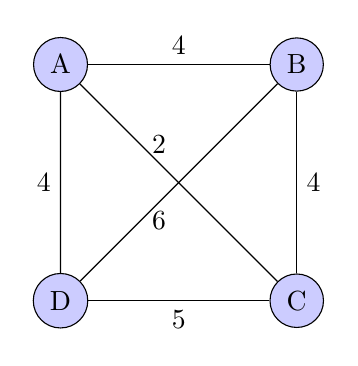
\begin{tikzpicture}[scale=3, every node/.style={circle, draw, fill=blue!20}]
			% Nodes
			\node (1) at (2,0) {D};
			\node (2) at (3,0) {C};
			\node (3) at (3,1) {B};
			\node (4) at (2,1) {A};
			% Edges with weights
			\draw (1) -- (2) node[midway, below, fill=none, draw=none, shape=rectangle] {5};
			\draw (2) -- (3) node[midway, right, fill=none, draw=none, shape=rectangle] {4};
			\draw (3) -- (4) node[midway, above, fill=none, draw=none, shape=rectangle] {4};
			\draw (4) -- (1) node[midway, left, fill=none, draw=none, shape=rectangle] {4};
			\draw (1) -- (3) node[pos = 0.4, below, fill=none, draw=none, shape=rectangle] {6};
			\draw (2) -- (4) node[pos = 0.6, above, fill=none, draw=none, shape=rectangle] {2};
		\end{tikzpicture}
	\end{center}
	
	\begin{equation*}
		w =  \{w_{AB},w_{AC},w_{AD},w_{BC},w_{CD},w_{BD}\} =  \{4,2,4,4,5,6\}
	\end{equation*}
	
	
	\subsection{Algorithm Construction}
	
	We will follow the instructions highlighted at the beginning of Chapter 3. Step 1 requires normalizing the edge weights. This involves sorting the edge weights in descending order, as specified in Equation \eqref{sorted-weights}:	
	
	\begin{equation*}
	w' = \{6,5,4,4,4,2\}
	\end{equation*}
	
	
	Next, we retrieve the sum $S$, as specified in Equation \eqref{sum-S}:
	\begin{equation*}
	S = \sum_{i=1}^{4} w'_i = 6 + 5  + 4 + 4 = 19
	\end{equation*}
	
	 We proceed to normalize our edge weights as described in Equation \eqref{normalization}, where we set $\epsilon = 1$.
	
	\begin{equation*}
		\tilde{w} = \frac{ \{4,2,4,4,5,6\}}{20} = \{0.2 , 0.1 , 0.2 , 0.2 , 0.25, 0.3\} 
	\end{equation*}
	
	
	
	
	\begin{center}	
		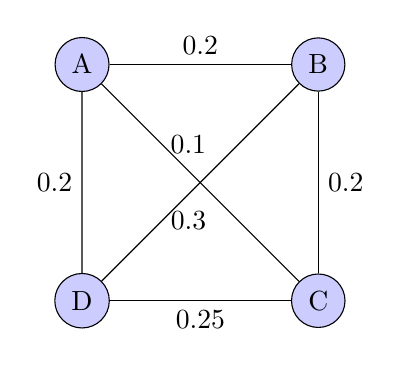
\begin{tikzpicture}[scale=3, every node/.style={circle, draw, fill=blue!20}]
			% Nodes
			\node (1) at (2,0) {D};
			\node (2) at (3,0) {C};
			\node (3) at (3,1) {B};
			\node (4) at (2,1) {A};
			% Edges with weights
			\draw (1) -- (2) node[midway, below, fill=none, draw=none, shape=rectangle] {0.25};
			\draw (2) -- (3) node[midway, right, fill=none, draw=none, shape=rectangle] {$0.2$};
			\draw (3) -- (4) node[midway, above, fill=none, draw=none, shape=rectangle] {$0.2$};
			\draw (4) -- (1) node[midway, left, fill=none, draw=none, shape=rectangle] {$0.2$};
			\draw (1) -- (3) node[pos = 0.4, below, xshift=1mm, fill=none, draw=none, shape=rectangle] {$0.3$};
			\draw (2) -- (4) node[pos = 0.6, above,xshift=1mm, fill=none, draw=none, shape=rectangle] {$0.1$};
		\end{tikzpicture}
	\end{center}
	
	
	Now, we move on to constructing the unitary operator and finding its corresponding eigenstates. The diagonals of matrices $U$ and $U'$ are as follows:
	
	
	\begin{align*}	
		u & = \begin{bmatrix}
			1 \\
			e^{i2\pi(0.2)} \\
			e^{i2\pi(0.1)} \\
			e^{i2\pi(0.2)} \\
		\end{bmatrix} 
		\otimes \begin{bmatrix}
			e^{i2\pi(0.2)} \\
			1 \\
			e^{i2\pi(0.2)} \\
			e^{i2\pi(0.3)} \\
		\end{bmatrix}
		\otimes \begin{bmatrix}
			e^{i2\pi(0.1)} \\
			e^{i2\pi(0.2)} \\
			1\\
			e^{i2\pi(0.25)} \\
		\end{bmatrix} 
		\otimes \begin{bmatrix}
		e^{i2\pi(0.2)} \\
		e^{i2\pi(0.3)} \\
		e^{i2\pi(0.25)} \\
			1 \\
		\end{bmatrix} 						 			
	\end{align*}
	
	\begin{align*}	
		u' & = \begin{bmatrix}
			1 \\
			e^{i2\pi(0.2)} \\
			e^{i2\pi(0.1)} \\
			e^{i2\pi(0.2)} \\
		\end{bmatrix} 
		\otimes \begin{bmatrix}
			e^{i2\pi(0.2)} \\
			1 \\
			e^{i2\pi(0.2)} \\
			e^{i2\pi(0)} \\
		\end{bmatrix}
		\otimes \begin{bmatrix}
			e^{i2\pi(0.1)} \\
			e^{i2\pi(0.2)} \\
			1\\
			e^{i2\pi(0.25)} \\
		\end{bmatrix} 
		\otimes \begin{bmatrix}
			e^{i2\pi(0.2)} \\
			e^{i2\pi(0)} \\
			e^{i2\pi(0.25)} \\
			1 \\
		\end{bmatrix} 						 			
	\end{align*}
	
To create our controlled matrices, we employ the block matrix structure illustrated in \ref{control-u-matrix}. Since both $U$ and $U'$ have $4^4$ diagonal elements, we require $8$ eigenstate qubits to represent all $256$ states.
	
	\begin{equation*}
		CU = \begin{bmatrix}
			\mathbb{I}_8 & 0 \\
			0 & U \\
		\end{bmatrix},\;\;\;
		CU' = \begin{bmatrix}
			\mathbb{I}_8 & 0 \\
			0 & U' \\
		\end{bmatrix}
	\end{equation*}
	
	
	Given our problem is symmetric, we can utilize the results and conversions provided in Table \ref{table:ham-cycle-details-4-city} for the first three cycles. Hence, we will estimate phases using the following eigenstates:
	
	$$|108\rangle = |01101100\rangle$$
	$$|114\rangle = |01110010\rangle$$
	$$|180\rangle = |10110100\rangle$$
	
	And we can anticipate the following phases:
	
	Cycle 1: $A \rightarrow B \rightarrow C \rightarrow D \rightarrow A$
	
	\begin{center}	
		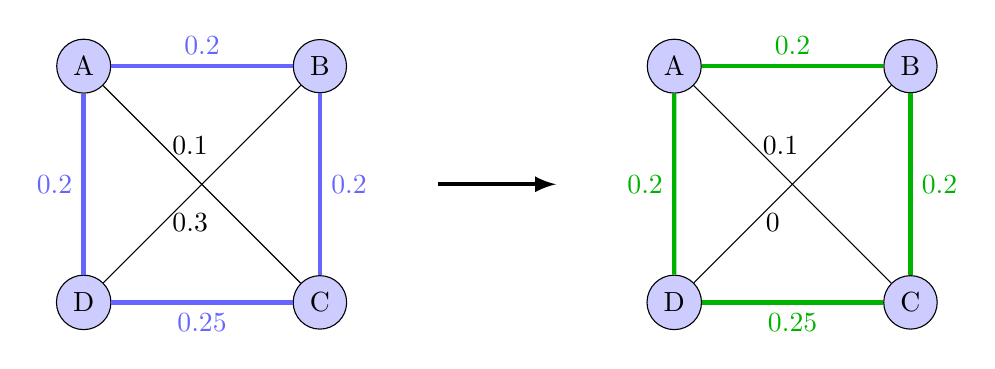
\begin{tikzpicture}[scale=3, every node/.style={circle, draw, fill=blue!20}]
			% Nodes
			\node (1) at (0,0) {D};
			\node (2) at (1,0) {C};
			\node (3) at (1,1) {B};
			\node (4) at (0,1) {A};
			% Edges with weights
			\draw[blue!60, ultra thick] (1) -- (2) node[midway, below, fill=none, draw=none, shape=rectangle] {$0.25$};
			\draw[blue!60,ultra  thick] (2) -- (3) node[midway, right, fill=none, draw=none, shape=rectangle] {$0.2$};
			\draw [blue!60, ultra thick](3) -- (4) node[midway, above, fill=none, draw=none, shape=rectangle] {$0.2$};
			\draw [blue!60,ultra  thick](4) -- (1) node[midway, left, fill=none, draw=none, shape=rectangle] {$0.2$};
			\draw (1) -- (3) node[pos = 0.4, xshift=1mm, below, fill=none, draw=none, shape=rectangle] {$0.3$};
			\draw (2) -- (4) node[pos = 0.6, xshift=1mm, above, fill=none, draw=none, shape=rectangle] {$0.1$};
			
			
			
			% Nodes
			\node (5) at (2.5,0) {D};
			\node (6) at (3.5,0) {C};
			\node (7) at (3.5,1) {B};
			\node (8) at (2.5,1) {A};
			% Edges with weights
			\draw[black!30!green, ultra thick] (5) -- (6) node[midway, below, fill=none, draw=none, shape=rectangle] {$0.25$};
			\draw[black!30!green, ultra thick] (6) -- (7) node[midway, right, fill=none, draw=none, shape=rectangle] {$0.2$};
			\draw [black!30!green, ultra thick](7) -- (8) node[midway, above, fill=none, draw=none, shape=rectangle] {$0.2$};
			\draw [black!30!green, ultra thick](8) -- (5) node[midway, left, fill=none, draw=none, shape=rectangle] {$0.2$};
			\draw (5) -- (7) node[pos = 0.4, below, fill=none, draw=none, shape=rectangle] {$0$};
			\draw (6) -- (8) node[pos = 0.6, xshift=1mm, above, fill=none, draw=none, shape=rectangle] {$0.1$};
			
			\draw[->, ultra thick, >=latex] (1.5, 0.5) -- (2, 0.5);
			
		\end{tikzpicture}
	\end{center}
	
	
	 $$u_{108} = e^{i2\pi (\gamma_{AB} + \gamma_{BC} + \gamma_{CD} + \gamma_{DA})} = e^{i2\pi(0.85)}$$
	 $$u'_{108} = e^{i2\pi (\gamma_{AB} + \gamma_{BC} + \gamma_{CD} + \gamma_{DA})} = e^{i2\pi(0.85)}$$
	 
	 
	 Cycle 2: $A \rightarrow B \rightarrow D \rightarrow C \rightarrow A$
	 
	 \begin{center}	
	 	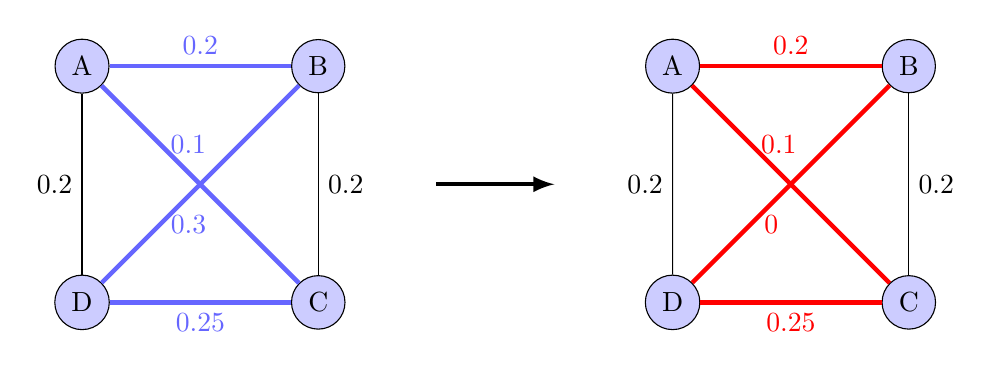
\begin{tikzpicture}[scale=3, every node/.style={circle, draw, fill=blue!20}]
	 		% Nodes
	 		\node (1) at (0,0) {D};
	 		\node (2) at (1,0) {C};
	 		\node (3) at (1,1) {B};
	 		\node (4) at (0,1) {A};
	 		% Edges with weights
	 		\draw [blue!60, ultra thick](1) -- (2) node[midway, below, fill=none, draw=none, shape=rectangle] {$0.25$};
	 		\draw (2) -- (3) node[midway, right, fill=none, draw=none, shape=rectangle] {$0.2$};
	 		\draw [blue!60, ultra thick](3) -- (4) node[midway, above, fill=none, draw=none, shape=rectangle] {$0.2$};
	 		\draw (4) -- (1) node[midway, left, fill=none, draw=none, shape=rectangle] {$0.2$};
	 		\draw [blue!60, ultra thick](1) -- (3) node[pos = 0.4, xshift=1mm, below, fill=none, draw=none, shape=rectangle] {$0.3$};
	 		\draw [blue!60, ultra thick](2) -- (4) node[pos = 0.6, xshift=1mm, above, fill=none, draw=none, shape=rectangle] {$0.1$};
	 		
	 		
	 		
	 		% Nodes
	 		\node (5) at (2.5,0) {D};
	 		\node (6) at (3.5,0) {C};
	 		\node (7) at (3.5,1) {B};
	 		\node (8) at (2.5,1) {A};
	 		% Edges with weights
	 		\draw[red, ultra thick] (5) -- (6) node[midway, below, fill=none, draw=none, shape=rectangle] {$0.25$};
	 		\draw (6) -- (7) node[midway, right, fill=none, draw=none, shape=rectangle] {$0.2$};
	 		\draw [red, ultra thick](7) -- (8) node[midway, above, fill=none, draw=none, shape=rectangle] {$0.2$};
	 		\draw (8) -- (5) node[midway, left, fill=none, draw=none, shape=rectangle] {$0.2$};
	 		\draw  [red, ultra thick](5) -- (7) node[pos = 0.4, below, fill=none, draw=none, shape=rectangle] {$0$};
	 		\draw  [red,ultra  thick](6) -- (8) node[pos = 0.6, xshift=1mm, above, fill=none, draw=none, shape=rectangle] {$0.1$};
	 		
	 		\draw[->, ultra thick, >=latex] (1.5, 0.5) -- (2, 0.5);
	 		
	 	\end{tikzpicture}
	 \end{center}
	 
	 $$ u_{114} = e^{i2\pi (\gamma_{AB} + \gamma_{BD} + \gamma_{DC} + \gamma_{CA})} = e^{i2\pi(0.85)}$$
	 $$ u'_{114} = e^{i2\pi (\gamma_{AB} + \gamma_{BD} + \gamma_{DC} + \gamma_{CA})} = e^{i2\pi(0.55)}$$
	 
	 
	 Cycle 3: $A \rightarrow C \rightarrow B \rightarrow D \rightarrow A$
	 
	 \begin{center}	
	 	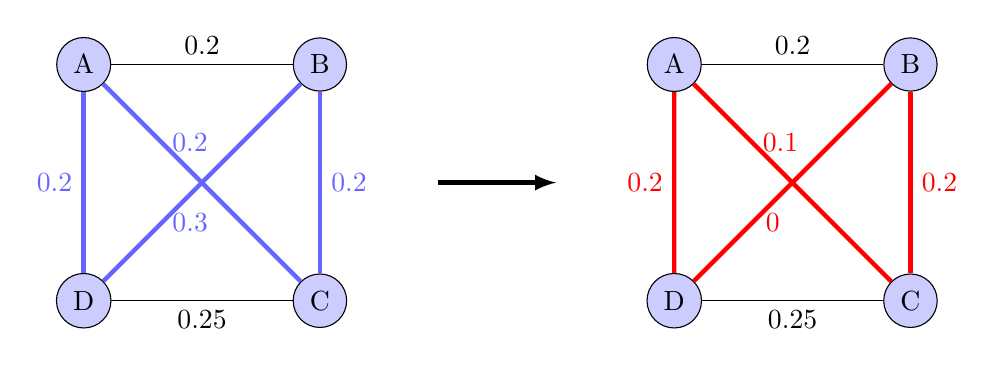
\begin{tikzpicture}[scale=3, every node/.style={circle, draw, fill=blue!20}]
	 		% Nodes
	 		\node (1) at (0,0) {D};
	 		\node (2) at (1,0) {C};
	 		\node (3) at (1,1) {B};
	 		\node (4) at (0,1) {A};
	 		% Edges with weights
	 		\draw (1) -- (2) node[midway, below, fill=none, draw=none, shape=rectangle] {$0.25$};
	 		\draw [blue!60, ultra thick](2) -- (3) node[midway, right, fill=none, draw=none, shape=rectangle] {$0.2$};
	 		\draw (3) -- (4) node[midway, above, fill=none, draw=none, shape=rectangle] {$0.2$};
	 		\draw [blue!60,ultra thick](4) -- (1) node[midway, left, fill=none, draw=none, shape=rectangle] {$0.2$};
	 		\draw [blue!60,ultra thick](1) -- (3) node[pos = 0.4, xshift=1mm, below, fill=none, draw=none, shape=rectangle] {$0.3$};
	 		\draw [blue!60,ultra thick](2) -- (4) node[pos = 0.6, xshift=1mm, above, fill=none, draw=none, shape=rectangle] {$0.2$};
	 		
	 		% Nodes
	 		\node (5) at (2.5,0) {D};
	 		\node (6) at (3.5,0) {C};
	 		\node (7) at (3.5,1) {B};
	 		\node (8) at (2.5,1) {A};
	 		% Edges with weights
	 		\draw (5) -- (6) node[midway, below, fill=none, draw=none, shape=rectangle] {$0.25$};
	 		\draw [red,ultra thick](6) -- (7) node[midway, right, fill=none, draw=none, shape=rectangle] {$0.2$};
	 		\draw (7) -- (8) node[midway, above, fill=none, draw=none, shape=rectangle] {$0.2$};
	 		\draw [red,ultra thick](8) -- (5) node[midway, left, fill=none, draw=none, shape=rectangle] {$0.2$};
	 		\draw  [red,ultra thick](5) -- (7) node[pos = 0.4, below, fill=none, draw=none, shape=rectangle] {$0$};
	 		\draw  [red,ultra thick](6) -- (8) node[pos = 0.6, xshift=1mm, above, fill=none, draw=none, shape=rectangle] {$0.1$};
	 		
	 		% Arrow pointing from the first graph to the second graph
	 		\draw[->, ultra thick, >=latex] (1.5, 0.5) -- (2, 0.5);
	 		
	 	\end{tikzpicture}
	 \end{center}
	 
	 $$ u_{180} = e^{i2\pi (\gamma_{AC} + \gamma_{CB} + \gamma_{BD} + \gamma_{DA})} = e^{i2\pi(0.80)}$$
	$$ u'_{180} = e^{i2\pi (\gamma_{AC} + \gamma_{CB} + \gamma_{BD} + \gamma_{DA})} = e^{i2\pi(0.50)}$$
	
	\subsection{Results: Simulations with Qiskit} \label{4-city-sim}
	
	We use Qiskit, an open-source quantum computing framework, for running simulations. Fig. \ref{fig:4-city-circuit} illustrates the circuit for our first Hamiltonian cycle initialized in the eigenstate $|01101100\rangle$. Similar circuits will be executed for the other two Hamiltonian cycles, with the only variation being the eigenstate initialization. Our simulations are ideal, implying that our results are not affected by noise. Each circuit is executed 1024 times by default, providing us with a quasi-probability distribution.
	


 \begin{figure}[!h]
		\centering
		\includegraphics[trim={8.5cm 4.4cm 6cm 4.4cm},clip, width=1 \linewidth]{"graphics/4-city-1-cycle-constrained-barrier"}
		\caption{The quantum circuit for the 4-city graph involves a 3-qubit phase estimation, measuring the Hamiltonian cycle $A \rightarrow B \rightarrow C \rightarrow D \rightarrow A$. The corresponding eigenstate is $|108\rangle = |01101100\rangle$, but due to Qiskit's convention on qubit ordering, the eigenstate is initialized in reverse. The CU gate represents the control unitary matrix containing all the Hamiltonian cycles. The CU' gate includes the same cycles, but before its construction, all edge weights not satisfying the condition ($< 6$) were set to zero. We have two sets of 3 qubits to be measured and stored in classical registers labelled 'output' and 'output c'.}
		\label{fig:4-city-circuit}
	\end{figure}		


	\begin{figure}[!h]
		\centering
		\includegraphics[width=\textwidth,height=0.9\textheight,keepaspectratio]{"graphics/3qubit-4city"}
		\caption{3-qubit phase estimation for the 4-city graph}
		\label{fig:4-city-graphic-3}
	\end{figure}		
	
		\begin{figure}[!h]
		\centering
		\includegraphics[ width=\textwidth,height=0.9\textheight,keepaspectratio]{"graphics/4qubit-4city"}
		\caption{4-qubit phase estimation for the 4-city graph}
		\label{fig:4-city-graphic-4}
	\end{figure}		
	
		\begin{figure}[!h]
		\centering
		\includegraphics[width=\textwidth,height=0.9\textheight,keepaspectratio]{"graphics/5qubit-4city"}
		\caption{5-qubit phase estimation for the 4-city graph}
		\label{fig:4-city-graphic-5}
	\end{figure}		
	
 We observe in Fig. \ref{fig:4-city-graphic-3} that our 3-qubit phase estimation for the first cycle with the highest counts yields $111\; 111$. The binary digits on the left correspond to the phase estimated after our condition is satisfied, while those on the right represent the estimation before. These binary digits can be converted to their decimal representation: 
 
 $$\mathrm{Cycle}\; 1: \;\; 0.111, \; 0.111 = 0.875, \; 0.875$$
 
 We can perform a similar analysis for the other two cycles:
 
 $$\mathrm{Cycle}\; 2: \;\; 0.100, \; 0.111 = 0.500, \; 0.875$$
 $$\mathrm{Cycle}\; 3: \;\; 0.110, \; 0.111 = 0.875, \; 0.750$$
 
 For each cycle, we can examine the two states with the highest counts and summarize them in Table \ref{table:sim-results-4-city}. This table also presents higher-order qubit estimations, namely $4$ and $5$.
 
\begin{table}[ht!]
	\centering
	\begin{tabular}{lllllll} % Updated for 7 columns
		\toprule
		Cycle & Expected & Phase Qubits & Highest Counts & Prob. & 2nd Highest Counts & Prob. \\
		\midrule
		\multirow{3}{*}{1} & \multirow{3}{*}{$0.85, \; 0.85$} & 3 & $0.875, \; 0.875$ & $77\%$ &  $0.75, \; 0.875$  & $6\%$ \\
		&                          & 4& $0.875, \; 0.875$ & $34\%$ &  $0.875, \; 0.8125$  & $16\%$ \\
		&                          & 5 & $0.84375, \; 0.84375$ & $77\%$ &  $0.84375, \; 0.875$  & $5\%$ \\
		\hline
		\multirow{3}{*}{2} & \multirow{3}{*}{$0.55, \; 0.85$} & 3 & $0.5, \; 0.875$ & $50\%$ &  $0.625, \; 0.875$  & $24\%$ \\
		&                          & 4& $0.5625, \; 0.875$ & $49\%$ &  $0.5625, \; 0.8125$  & $24\%$ \\
		&                          & 5 & $0.5625, \; 0.84375$ & $51\%$ &  $0.53125, \; 0.84375$  & $21\%$ \\
		\hline
		\multirow{3}{*}{3} & \multirow{3}{*}{$0.50, \; 0.80$ } & 3 & $0.5, \; 0.75$ & $58\%$ &  $0.5, \; 0.875$  & $27\%$ \\
		&                          & 4& $0.5, \; 0.8125$ & $88\%$ &  $0.5, \; 0.75$  & $6\%$ \\
		&                          & 5 & $0.5, \; 0.8125$ & $58\%$ &  $0.5, \; 0.78125$  & $26\%$ \\
		\bottomrule
	\end{tabular}
	\caption{Simulation results for the 4-city graph.}
	\label{table:sim-results-4-city}
\end{table} 

\clearpage


\section{An Undirected 5-City Graph}

	Let us consider the following example of a symmetric 5-city system. In this undirected graph, we need to look at $(5-1)!/2 = 12$ Hamiltonian cycles. The condition for our BTSP in this case will involve finding a Hamiltonian cycle where all edge weights are $ < 9$:
	
	
	\begin{center}	
		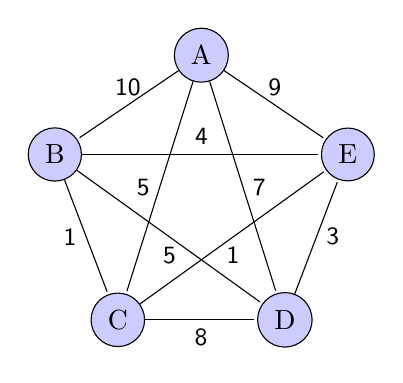
\begin{tikzpicture}[-,shorten >=1pt,auto,node distance=1.5cm,main node/.style={circle, draw, fill=blue!20}]
			
			\node[main node] (1) {A};
			\node[main node] (2) [below left of=1, xshift = -0.8cm, yshift = -0.2cm] {B};
			\node[main node] (3) [below of=2, xshift= 0.8cm, yshift = -0.6cm] {C};
			\node[main node] (5) [below right of=1, xshift = 0.8cm, yshift = -0.2cm] {E};
			\node[main node] (4) [below of=5, xshift= -0.8cm, yshift = -0.6cm] {D};
			
			
			
			\path[every node/.style={font=\sffamily\small}]
			(1)
			edge node [right] {7} (4)
			edge node[above] {10} (2)
			edge node[left] {5} (3)
			edge node[above] {9} (5)
			
			(2) 
			edge node[below] {5} (4)
			edge node[left] {1} (3)
			edge node[above] {4} (5)
			
			(3)
			edge node[below] {8} (4)
			edge node[below] {1} (5)
			
			(4) edge node[right] {3} (5);
			
		\end{tikzpicture}
		
	\end{center}
	
	
		\subsection{Algorithm Construction}
	
	We will follow the instructions highlighted at the beginning of Chapter 3. Step 1 requires normalizing the edge weights. This involves sorting the edge weights in descending order, as specified in Equation \eqref{sorted-weights}:	
	
	\begin{equation*}
		w' = \{10,9,8,7,5,5,4,3,1,1\}
	\end{equation*}
	
	
	Next, we retrieve the sum $S$, as specified in Equation \eqref{sum-S}:
	\begin{equation*}
		S = \sum_{i=1}^{5} w'_i = 10 + 9  + 8 + 7 + 5 = 39
	\end{equation*}
	
	 We proceed to normalize our edge weights as described in Equation \eqref{normalization}, where we set $\epsilon = 1$.
	
	\begin{equation*}
		\tilde{w} = \frac{  \{10,9,8,7,5,5,4,3,1,1\}}{40} = \{0.25 , 0.225 , 0.2 , 0.175 , 0.125, 0.125, 0.1, 0.075, 0.025, 0.025\} 
	\end{equation*}
	
	
	\begin{center}	
		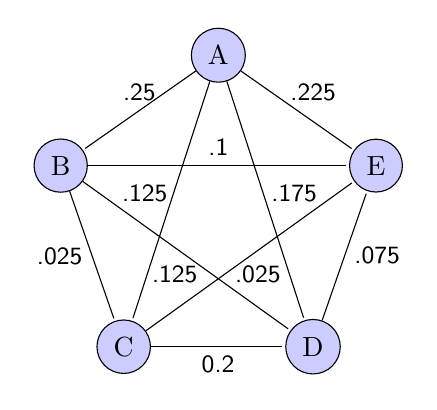
\begin{tikzpicture}[-,shorten >=1pt,auto,node distance=1.7cm,main node/.style={circle, draw, fill=blue!20}]
			
			\node[main node] (1) {A};
			\node[main node] (2) [below left of=1, xshift = -0.8cm, yshift = -0.2cm] {B};
			\node[main node] (3) [below of=2, xshift= 0.8cm, yshift = -0.6cm] {C};
			\node[main node] (5) [below right of=1, xshift = 0.8cm, yshift = -0.2cm] {E};
			\node[main node] (4) [below of=5, xshift= -0.8cm, yshift = -0.6cm] {D};
			
			
			
			\path[every node/.style={font=\sffamily\small}]
			(1)
			edge node [right, yshift = 0.1cm, xshift = -0.05cm] {.175} (4)
			edge node[above] {.25} (2)
			edge node[left, yshift = 0.1cm, xshift = 0.08cm] {.125} (3)
			edge node[above, xshift = 0.2cm] {.225} (5)
			
			(2) 
			edge node[below, xshift = -0.15cm] {.125} (4)
			edge node[left] {.025} (3)
			edge node[above] {.1} (5)
			
			(3)
			edge node[below] {0.2} (4)
			edge node[below, xshift = 0.1cm] {.025} (5)
			
			(4) edge node[right] {.075} (5);
			
		\end{tikzpicture}
		
	\end{center}
	
		Now, we move on to constructing the unitary operator and finding its corresponding eigenstates. The diagonals of matrices $U$ and $U'$ are as follows:
	
	
	\begin{align*}	
		u & = \begin{bmatrix}
			1 \\
			e^{i2\pi(0.25)} \\
			e^{i2\pi(0.125)} \\
			e^{i2\pi(0.175)} \\
			e^{i2\pi(0.225)} \\
		\end{bmatrix} 
		\otimes \begin{bmatrix}
			e^{i2\pi(0.25)} \\
			1 \\
			e^{i2\pi(0.025)} \\
			e^{i2\pi(0.125)} \\
			e^{i2\pi(0.1)} \\
		\end{bmatrix}
		\otimes \begin{bmatrix}
			e^{i2\pi(0.125)} \\
			e^{i2\pi(0.025)} \\
			1\\
			e^{i2\pi(0.2)} \\
			e^{i2\pi(0.025)} \\
		\end{bmatrix} 
		\otimes \begin{bmatrix}
			e^{i2\pi(0.175)} \\
			e^{i2\pi(0.125)} \\
			e^{i2\pi(0.2)} \\
			1 \\
			e^{i2\pi(0.075)} \\
		\end{bmatrix} 
		\otimes \begin{bmatrix}
			e^{i2\pi(0.225)} \\
			e^{i2\pi(0.1)} \\
			e^{i2\pi(0.025)} \\
			e^{i2\pi(0.075)} \\
			1 \\
		\end{bmatrix} 							 			
	\end{align*}
	
	\begin{align*}	
	u' & = \begin{bmatrix}
		1 \\
		e^{i2\pi(0)} \\
		e^{i2\pi(0.125)} \\
		e^{i2\pi(0.175)} \\
		e^{i2\pi(0)} \\
	\end{bmatrix} 
	\otimes \begin{bmatrix}
		e^{i2\pi(0)} \\
		1 \\
		e^{i2\pi(0.025)} \\
		e^{i2\pi(0.125)} \\
		e^{i2\pi(0.1)} \\
	\end{bmatrix}
	\otimes \begin{bmatrix}
		e^{i2\pi(0.125)} \\
		e^{i2\pi(0.025)} \\
		1\\
		e^{i2\pi(0.2)} \\
		e^{i2\pi(0.025)} \\
	\end{bmatrix} 
	\otimes \begin{bmatrix}
		e^{i2\pi(0.175)} \\
		e^{i2\pi(0.125)} \\
		e^{i2\pi(0.2)} \\
		1 \\
		e^{i2\pi(0.075)} \\
	\end{bmatrix} 
	\otimes \begin{bmatrix}
		e^{i2\pi(0)} \\
		e^{i2\pi(0.1)} \\
		e^{i2\pi(0.025)} \\
		e^{i2\pi(0.075)} \\
		1 \\
	\end{bmatrix} 							 			
\end{align*}
	

	
	The number of diagonal elements in $U$ and $U'$ is $5^5 = 3125$, thus we need at least $12$ eigenstate qubits to represent all $3125$ states. We will have left over states ($2^{12} - 5^5 = 971$). To accomodate this issue we need to add $1$'s to the end of the diagonal of matrices $U$ and $U'$. With this method, we do not affect the eigenstates.
	

	
	\begin{equation}\label{ones}
	\mathrm{diag}(U) = [u, \mathrm{ones}(971)], \;\; \mathrm{diag}(U') = [u', \mathrm{ones}(971)]
	\end{equation}
	
	Now we can create our controlled matrices. We employ the block matrix structure illustrated in \ref{control-u-matrix}. We require $12$ eigenstate qubits to represent all $256$ states.
	
\begin{equation*}
	CU = \begin{bmatrix}
		\mathbb{I}_{12} & 0 \\
		0 & U \\
	\end{bmatrix},\;\;\;
	CU' = \begin{bmatrix}
		\mathbb{I}_{12} & 0 \\
		0 & U' \\
	\end{bmatrix}
\end{equation*}	
	
		Given our problem is symmetric, we can utilize half of the results and conversions provided in Table \ref{table:ham-cycle-details-5-city}. Hence, we will estimate phases using the following eigenstates:
	
	$$|970\rangle  = |001111001010\rangle$$
	$$|978\rangle  = |001111010010\rangle$$
	$$|1110\rangle = |010001010110\rangle$$
	$$|1022\rangle = |001111111110\rangle$$
	$$|1202\rangle = |010010110010\rangle$$
	$$|1138\rangle = |010001110010\rangle$$
	$$|1670\rangle = |011010000110\rangle$$
	$$|1778\rangle = |011011110010\rangle$$
	$$|1830\rangle = |011100100110\rangle$$
	$$|1726\rangle = |011010111110\rangle$$
	$$|2230\rangle = |100010110110\rangle$$
	$$|2410\rangle = |100101101010\rangle$$
	
	And we can anticipate the following phases:
	\clearpage
	
		Cycle 1: $A \rightarrow B \rightarrow C \rightarrow D \rightarrow E \rightarrow A$.\;\;\;\;\;\;\;\;\;\;\;\;\;\; $u_{970}  = e^{i2\pi(0.775)}$, \;\;\;\;\;$u'_{970} = e^{i2\pi(0.3)}$
		
	\begin{center}	
		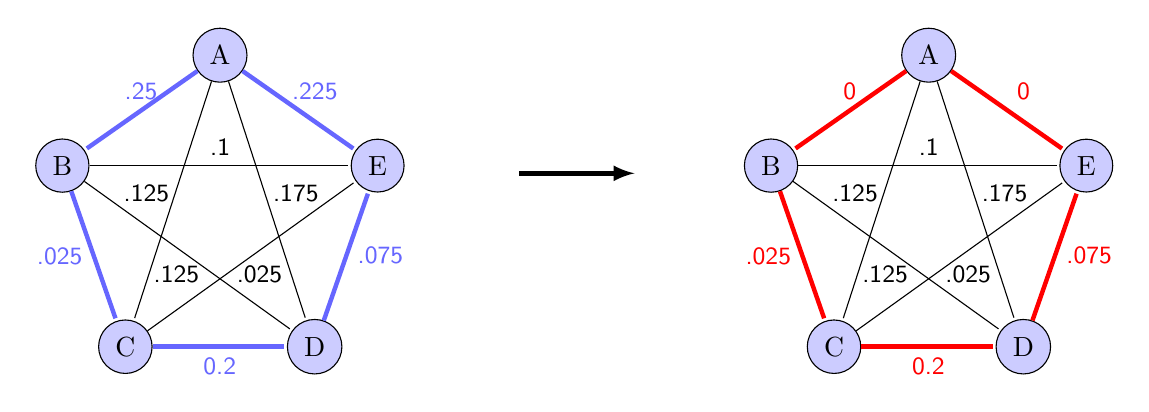
\begin{tikzpicture}[-,shorten >=1pt,auto,node distance=1.7cm,main node/.style={circle, draw, fill=blue!20}]
			% Nodes
			\node [main node] (1) at (0,0) {A};
			\node[main node] (2) [below left of=1, xshift = -0.8cm, yshift = -0.2cm] {B};
			\node[main node] (3) [below of=2, xshift= 0.8cm, yshift = -0.6cm] {C};
			\node[main node] (5) [below right of=1, xshift = 0.8cm, yshift = -0.2cm] {E};
			\node[main node] (4) [below of=5, xshift= -0.8cm, yshift = -0.6cm] {D};
			
			
			
			\path[every node/.style={font=\sffamily\small}]
			(1)
			edge node [right, yshift = 0.1cm, xshift = -0.05cm] {.175} (4)
			edge[blue!60,ultra thick] node[above] {.25} (2)
			edge node[left, yshift = 0.1cm, xshift = 0.08cm] {.125} (3)
			edge[blue!60,ultra thick] node[above, xshift = 0.2cm] {.225} (5)
			
			(2) 
			edge node[below, xshift = -0.15cm] {.125} (4)
			edge[blue!60,ultra thick] node[left] {.025} (3)
			edge node[above] {.1} (5)
			
			(3)
			edge[blue!60,ultra thick] node[below] {0.2} (4)
			edge node[below, xshift = 0.1cm] {.025} (5)
			
			(4) edge [blue!60,ultra thick] node[right] {.075} (5);
			
			\node [main node] (6) at (9,0) {A};
			\node[main node] (7) [below left of=6, xshift = -0.8cm, yshift = -0.2cm] {B};
			\node[main node] (8) [below of=7, xshift= 0.8cm, yshift = -0.6cm] {C};
			\node[main node] (10) [below right of=6, xshift = 0.8cm, yshift = -0.2cm] {E};
			\node[main node] (9) [below of=10, xshift= -0.8cm, yshift = -0.6cm] {D};
			
			
			\path[every node/.style={font=\sffamily\small}]
			(6)
			edge node [right, yshift = 0.1cm, xshift = -0.05cm] {.175} (9)
			edge [red,ultra thick]node[above] {0} (7)
			edgenode[left, yshift = 0.1cm, xshift = 0.08cm] {.125} (8)
			edge[red,ultra thick] node[above, xshift = 0.2cm] {0} (10)
			
			(7) 
			edge node[below, xshift = -0.15cm] {.125} (9)
			edge[red,ultra thick] node[left] {.025} (8)
			edge node[above] {.1} (10)
			
			(8)
			edge [red,ultra thick] node[below] {0.2} (9)
			edge node[below, xshift = 0.1cm] {.025} (10)
			
			(9)edge[red,ultra thick]  node[right] {.075} (10);
			
			\draw[->, ultra thick, >=latex] (3.8, -1.5) -- (5.3, -1.5);
			
		\end{tikzpicture}
	\end{center}
	
	Cycle 2: $A \rightarrow B \rightarrow C \rightarrow E \rightarrow D \rightarrow A$.\;\;\;\;\;\;\;\;\;\;\;\;\;\; $ u_{978}  = e^{i2\pi(0.55)}$, \;\;\;\;\; $ u'_{978} = e^{i2\pi(0.3)}$
	\begin{center}	
		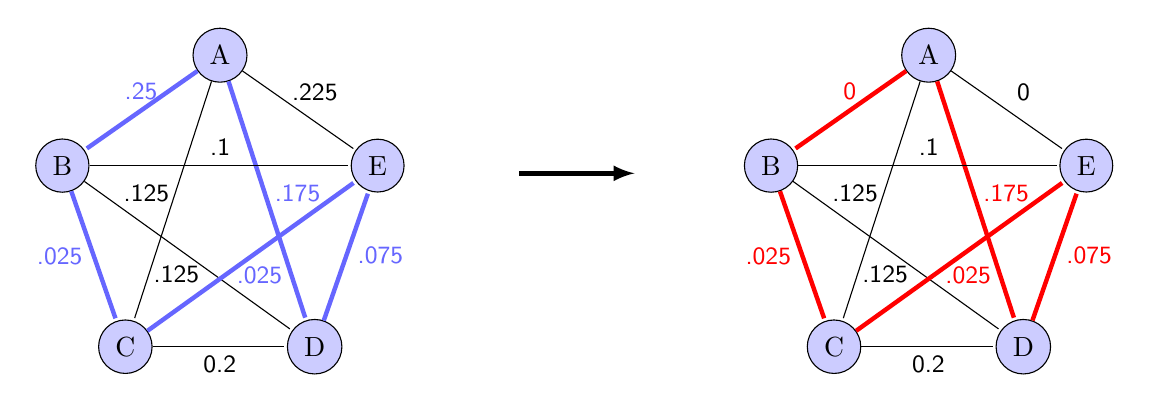
\begin{tikzpicture}[-,shorten >=1pt,auto,node distance=1.7cm,main node/.style={circle, draw, fill=blue!20}]
			% Nodes
			\node [main node] (1) at (0,0) {A};
			\node[main node] (2) [below left of=1, xshift = -0.8cm, yshift = -0.2cm] {B};
			\node[main node] (3) [below of=2, xshift= 0.8cm, yshift = -0.6cm] {C};
			\node[main node] (5) [below right of=1, xshift = 0.8cm, yshift = -0.2cm] {E};
			\node[main node] (4) [below of=5, xshift= -0.8cm, yshift = -0.6cm] {D};
			
			
			
			\path[every node/.style={font=\sffamily\small}]
			(1)
			edge [blue!60,ultra thick]node [right, yshift = 0.1cm, xshift = -0.05cm] {.175} (4)
			edge [blue!60,ultra thick]node[above] {.25} (2)
			edge node[left, yshift = 0.1cm, xshift = 0.08cm] {.125} (3)
			edge node[above, xshift = 0.2cm] {.225} (5)
			
			(2) 
			edge node[below, xshift = -0.15cm] {.125} (4)
			edge [blue!60,ultra thick]node[left] {.025} (3)
			edge node[above] {.1} (5)
			
			(3)
			edge node[below] {0.2} (4)
			edge [blue!60,ultra thick]node[below, xshift = 0.1cm] {.025} (5)
			
			(4) edge[blue!60,ultra thick] node[right] {.075} (5);
			
			\node [main node] (6) at (9,0) {A};
			\node[main node] (7) [below left of=6, xshift = -0.8cm, yshift = -0.2cm] {B};
			\node[main node] (8) [below of=7, xshift= 0.8cm, yshift = -0.6cm] {C};
			\node[main node] (10) [below right of=6, xshift = 0.8cm, yshift = -0.2cm] {E};
			\node[main node] (9) [below of=10, xshift= -0.8cm, yshift = -0.6cm] {D};
			
			
			\path[every node/.style={font=\sffamily\small}]
			(6)
			edge [red,ultra thick] node [right, yshift = 0.1cm, xshift = -0.05cm] {.175} (9)
			edge[red,ultra thick] node[above] {0} (7)
			edge node[left, yshift = 0.1cm, xshift = 0.08cm] {.125} (8)
			edge node[above, xshift = 0.2cm] {0} (10)
			
			(7) 
			edge node[below, xshift = -0.15cm] {.125} (9)
			edge [red,ultra thick]node[left] {.025} (8)
			edge node[above] {.1} (10)
			
			(8)
			edge node[below] {0.2} (9)
			edge[red,ultra thick] node[below, xshift = 0.1cm] {.025} (10)
			
			(9)  edge [red,ultra thick] node[right] {.075} (10);
			
			\draw[->, ultra thick, >=latex] (3.8, -1.5) -- (5.3, -1.5);
			
		\end{tikzpicture}
	\end{center}

	
	Cycle 3: $A \rightarrow B \rightarrow D \rightarrow C \rightarrow E \rightarrow A$.\;\;\;\;\;\;\;\;\;\;\;\;\;\; $ u_{1110}  = e^{i2\pi(0.825)}$, \;\;\;\;\; $ u'_{1110} = e^{i2\pi(0.35)}$
	\begin{center}	
		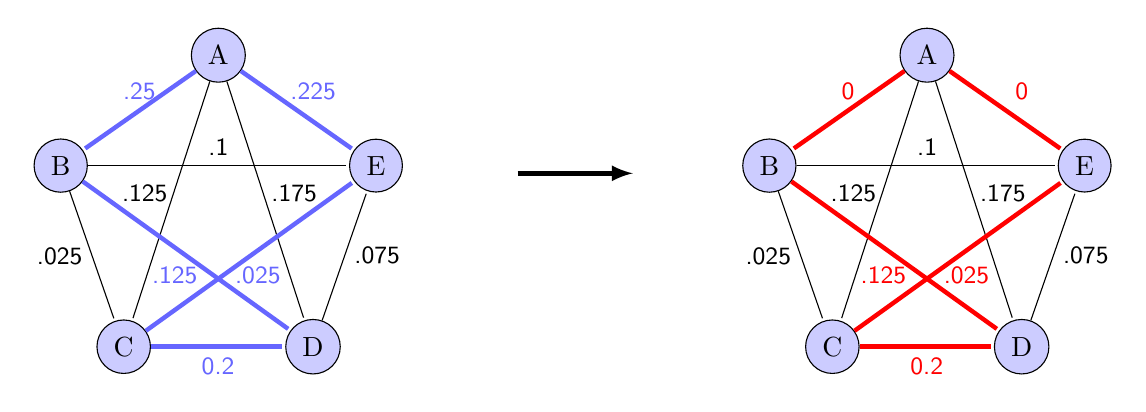
\begin{tikzpicture}[-,shorten >=1pt,auto,node distance=1.7cm,main node/.style={circle, draw, fill=blue!20}]
			% Nodes
			\node [main node] (1) at (0,0) {A};
			\node[main node] (2) [below left of=1, xshift = -0.8cm, yshift = -0.2cm] {B};
			\node[main node] (3) [below of=2, xshift= 0.8cm, yshift = -0.6cm] {C};
			\node[main node] (5) [below right of=1, xshift = 0.8cm, yshift = -0.2cm] {E};
			\node[main node] (4) [below of=5, xshift= -0.8cm, yshift = -0.6cm] {D};
			
			
			
			\path[every node/.style={font=\sffamily\small}]
			(1)
			edge node [right, yshift = 0.1cm, xshift = -0.05cm] {.175} (4)
			edge [blue!60,ultra thick] node[above] {.25} (2)
			edge node[left, yshift = 0.1cm, xshift = 0.08cm] {.125} (3)
			edge[blue!60,ultra thick] node[above, xshift = 0.2cm] {.225} (5)
			
			(2) 
			edge[blue!60,ultra thick] node[below, xshift = -0.15cm] {.125} (4)
			edge node[left] {.025} (3)
			edge node[above] {.1} (5)
			
			(3)
			edge[blue!60,ultra thick] node[below] {0.2} (4)
			edge [blue!60,ultra thick]node[below, xshift = 0.1cm] {.025} (5)
			
			(4) edge node[right] {.075} (5);
			
			\node [main node] (6) at (9,0) {A};
			\node[main node] (7) [below left of=6, xshift = -0.8cm, yshift = -0.2cm] {B};
			\node[main node] (8) [below of=7, xshift= 0.8cm, yshift = -0.6cm] {C};
			\node[main node] (10) [below right of=6, xshift = 0.8cm, yshift = -0.2cm] {E};
			\node[main node] (9) [below of=10, xshift= -0.8cm, yshift = -0.6cm] {D};
			
			
			\path[every node/.style={font=\sffamily\small}]
			(6)
			edge node [right, yshift = 0.1cm, xshift = -0.05cm] {.175} (9)
			edge[red,ultra thick] node[above] {0} (7)
			edge node[left, yshift = 0.1cm, xshift = 0.08cm] {.125} (8)
			edge[red,ultra thick] node[above, xshift = 0.2cm] {0} (10)
			
			(7) 
			edge [red,ultra thick]node[below, xshift = -0.15cm] {.125} (9)
			edge node[left] {.025} (8)
			edge node[above] {.1} (10)
			
			(8)
			edge[red,ultra thick] node[below] {0.2} (9)
			edge[red,ultra thick] node[below, xshift = 0.1cm] {.025} (10)
			
			(9) edge node[right] {.075} (10);
			
			\draw[->, ultra thick, >=latex] (3.8, -1.5) -- (5.3, -1.5);
			
		\end{tikzpicture}
	\end{center}
	
		Cycle 4: $A \rightarrow B \rightarrow D \rightarrow E \rightarrow C \rightarrow A$.\;\;\;\;\;\;\;\;\;\;\;\;\;\; $ u_{1022}  = e^{i2\pi(0.6)}$, \;\;\;\;\; $ u'_{1022} = e^{i2\pi(0.35)}$
	\begin{center}	
		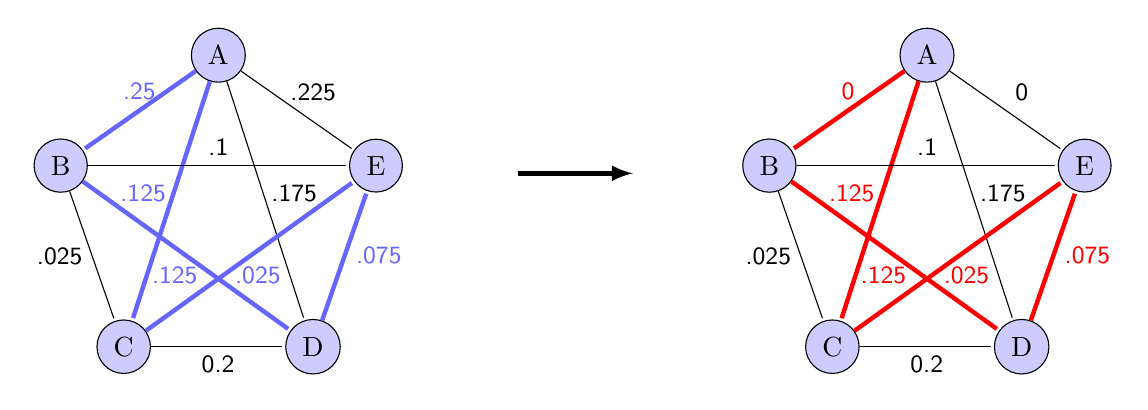
\begin{tikzpicture}[-,shorten >=1pt,auto,node distance=1.7cm,main node/.style={circle, draw, fill=blue!20}]
			% Nodes
			\node [main node] (1) at (0,0) {A};
			\node[main node] (2) [below left of=1, xshift = -0.8cm, yshift = -0.2cm] {B};
			\node[main node] (3) [below of=2, xshift= 0.8cm, yshift = -0.6cm] {C};
			\node[main node] (5) [below right of=1, xshift = 0.8cm, yshift = -0.2cm] {E};
			\node[main node] (4) [below of=5, xshift= -0.8cm, yshift = -0.6cm] {D};
			
			
			
			\path[every node/.style={font=\sffamily\small}]
			(1)
			edge node [right, yshift = 0.1cm, xshift = -0.05cm] {.175} (4)
			edge[blue!60,ultra thick] node[above] {.25} (2)
			edge [blue!60,ultra thick] node[left, yshift = 0.1cm, xshift = 0.08cm] {.125} (3)
			edge node[above, xshift = 0.2cm] {.225} (5)
			
			(2) 
			edge [blue!60,ultra thick]node[below, xshift = -0.15cm] {.125} (4)
			edge node[left] {.025} (3)
			edge node[above] {.1} (5)
			
			(3)
			edge node[below] {0.2} (4)
			edge [blue!60,ultra thick]node[below, xshift = 0.1cm] {.025} (5)
			
			(4) edge [blue!60,ultra thick]node[right] {.075} (5);
			
			\node [main node] (6) at (9,0) {A};
			\node[main node] (7) [below left of=6, xshift = -0.8cm, yshift = -0.2cm] {B};
			\node[main node] (8) [below of=7, xshift= 0.8cm, yshift = -0.6cm] {C};
			\node[main node] (10) [below right of=6, xshift = 0.8cm, yshift = -0.2cm] {E};
			\node[main node] (9) [below of=10, xshift= -0.8cm, yshift = -0.6cm] {D};
			
			
			\path[every node/.style={font=\sffamily\small}]
			(6)
			edge node [right, yshift = 0.1cm, xshift = -0.05cm] {.175} (9)
			edge [red,ultra thick]node[above] {0} (7)
			edge [red,ultra thick]node[left, yshift = 0.1cm, xshift = 0.08cm] {.125} (8)
			edge node[above, xshift = 0.2cm] {0} (10)
			
			(7) 
			edge [red,ultra thick]node[below, xshift = -0.15cm] {.125} (9)
			edge node[left] {.025} (8)
			edge node[above] {.1} (10)
			
			(8)
			edge node[below] {0.2} (9)
			edge[red,ultra thick] node[below, xshift = 0.1cm] {.025} (10)
			
			(9) edge [red,ultra thick]node[right] {.075} (10);
			
			\draw[->, ultra thick, >=latex] (3.8, -1.5) -- (5.3, -1.5);
			
		\end{tikzpicture}
	\end{center}
	
		Cycle 5: $A \rightarrow B \rightarrow E \rightarrow C \rightarrow D \rightarrow A$.\;\;\;\;\;\;\;\;\;\;\;\;\;\; $ u_{1202}  = e^{i2\pi(0.75)}$, \;\;\;\;\; $ u'_{1202} = e^{i2\pi(0.5)}$
	\begin{center}	
		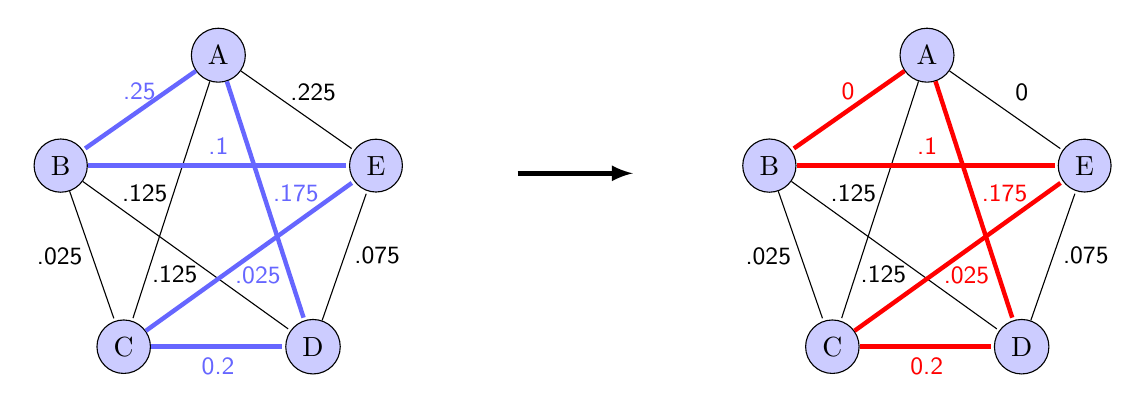
\begin{tikzpicture}[-,shorten >=1pt,auto,node distance=1.7cm,main node/.style={circle, draw, fill=blue!20}]
			% Nodes
			\node [main node] (1) at (0,0) {A};
			\node[main node] (2) [below left of=1, xshift = -0.8cm, yshift = -0.2cm] {B};
			\node[main node] (3) [below of=2, xshift= 0.8cm, yshift = -0.6cm] {C};
			\node[main node] (5) [below right of=1, xshift = 0.8cm, yshift = -0.2cm] {E};
			\node[main node] (4) [below of=5, xshift= -0.8cm, yshift = -0.6cm] {D};
			
			
			
			\path[every node/.style={font=\sffamily\small}]
			(1)
			edge  [blue!60,ultra thick]node [right, yshift = 0.1cm, xshift = -0.05cm] {.175} (4)
			edge [blue!60,ultra thick] node[above] {.25} (2)
			edge node[left, yshift = 0.1cm, xshift = 0.08cm] {.125} (3)
			edge node[above, xshift = 0.2cm] {.225} (5)
			
			(2) 
			edge node[below, xshift = -0.15cm] {.125} (4)
			edge node[left] {.025} (3)
			edge  [blue!60,ultra thick]node[above] {.1} (5)
			
			(3)
			edge  [blue!60,ultra thick]node[below] {0.2} (4)
			edge  [blue!60,ultra thick]node[below, xshift = 0.1cm] {.025} (5)
			
			(4) edge node[right] {.075} (5);
			
			\node [main node] (6) at (9,0) {A};
			\node[main node] (7) [below left of=6, xshift = -0.8cm, yshift = -0.2cm] {B};
			\node[main node] (8) [below of=7, xshift= 0.8cm, yshift = -0.6cm] {C};
			\node[main node] (10) [below right of=6, xshift = 0.8cm, yshift = -0.2cm] {E};
			\node[main node] (9) [below of=10, xshift= -0.8cm, yshift = -0.6cm] {D};
			
			
			\path[every node/.style={font=\sffamily\small}]
			(6)
			edge[red,ultra thick] node [right, yshift = 0.1cm, xshift = -0.05cm] {.175} (9)
			edge[red,ultra thick] node[above] {0} (7)
			edge node[left, yshift = 0.1cm, xshift = 0.08cm] {.125} (8)
			edge node[above, xshift = 0.2cm] {0} (10)
			
			(7) 
			edge node[below, xshift = -0.15cm] {.125} (9)
			edge node[left] {.025} (8)
			edge[red,ultra thick] node[above] {.1} (10)
			
			(8)
			edge [red,ultra thick]node[below] {0.2} (9)
			edge [red,ultra thick]node[below, xshift = 0.1cm] {.025} (10)
			
			(9) edge node[right] {.075} (10);
			
			\draw[->, ultra thick, >=latex] (3.8, -1.5) -- (5.3, -1.5);
			
		\end{tikzpicture}
	\end{center}
	
		Cycle 6: $A \rightarrow B \rightarrow E \rightarrow D \rightarrow C \rightarrow A$.\;\;\;\;\;\;\;\;\;\;\;\;\;\; $ u_{1138}  = e^{i2\pi(0.75)}$, \;\;\;\;\; $ u'_{1138} = e^{i2\pi(0.5)}$
	\begin{center}	
		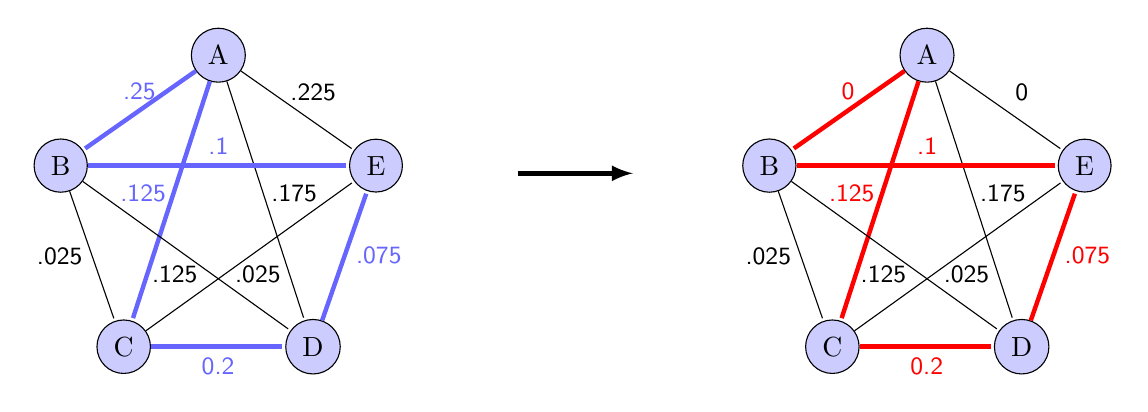
\begin{tikzpicture}[-,shorten >=1pt,auto,node distance=1.7cm,main node/.style={circle, draw, fill=blue!20}]
			% Nodes
			\node [main node] (1) at (0,0) {A};
			\node[main node] (2) [below left of=1, xshift = -0.8cm, yshift = -0.2cm] {B};
			\node[main node] (3) [below of=2, xshift= 0.8cm, yshift = -0.6cm] {C};
			\node[main node] (5) [below right of=1, xshift = 0.8cm, yshift = -0.2cm] {E};
			\node[main node] (4) [below of=5, xshift= -0.8cm, yshift = -0.6cm] {D};
			
			
			
			\path[every node/.style={font=\sffamily\small}]
			(1)
			edge node [right, yshift = 0.1cm, xshift = -0.05cm] {.175} (4)
			edge [blue!60,ultra thick] node[above] {.25} (2)
			edge[blue!60,ultra thick]  node[left, yshift = 0.1cm, xshift = 0.08cm] {.125} (3)
			edge node[above, xshift = 0.2cm] {.225} (5)
			
			(2) 
			edge node[below, xshift = -0.15cm] {.125} (4)
			edge node[left] {.025} (3)
			edge  [blue!60,ultra thick] node[above] {.1} (5)
			
			(3)
			edge [blue!60,ultra thick]  node[below] {0.2} (4)
			edge node[below, xshift = 0.1cm] {.025} (5)
			
			(4)  edge[blue!60,ultra thick]  node[right] {.075} (5);
			
			\node [main node] (6) at (9,0) {A};
			\node[main node] (7) [below left of=6, xshift = -0.8cm, yshift = -0.2cm] {B};
			\node[main node] (8) [below of=7, xshift= 0.8cm, yshift = -0.6cm] {C};
			\node[main node] (10) [below right of=6, xshift = 0.8cm, yshift = -0.2cm] {E};
			\node[main node] (9) [below of=10, xshift= -0.8cm, yshift = -0.6cm] {D};
			
			
			\path[every node/.style={font=\sffamily\small}]
			(6)
			edge node [right, yshift = 0.1cm, xshift = -0.05cm] {.175} (9)
			edge[red,ultra thick] node[above] {0} (7)
			edge [red,ultra thick]node[left, yshift = 0.1cm, xshift = 0.08cm] {.125} (8)
			edge node[above, xshift = 0.2cm] {0} (10)
			
			(7) 
			edge node[below, xshift = -0.15cm] {.125} (9)
			edge node[left] {.025} (8)
			edge [red,ultra thick]node[above] {.1} (10)
			
			(8)
			edge[red,ultra thick] node[below] {0.2} (9)
			edge node[below, xshift = 0.1cm] {.025} (10)
			
			(9) edge[red,ultra thick] node[right] {.075} (10);
			
			\draw[->, ultra thick, >=latex] (3.8, -1.5) -- (5.3, -1.5);
			
		\end{tikzpicture}
	\end{center}
	
		Cycle 7: $A \rightarrow C \rightarrow B \rightarrow D \rightarrow E \rightarrow A$.\;\;\;\;\;\;\;\;\;\;\;\;\;\; $ u_{1670}  = e^{i2\pi(0.575)}$, \;\;\;\;\; $ u'_{1670} = e^{i2\pi(0.35)}$
	\begin{center}	
		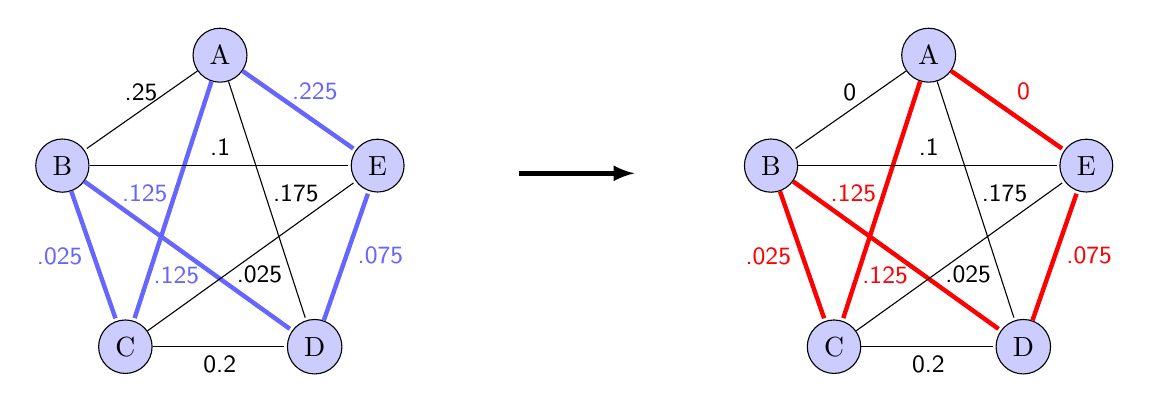
\begin{tikzpicture}[-,shorten >=1pt,auto,node distance=1.7cm,main node/.style={circle, draw, fill=blue!20}]
			% Nodes
			\node [main node] (1) at (0,0) {A};
			\node[main node] (2) [below left of=1, xshift = -0.8cm, yshift = -0.2cm] {B};
			\node[main node] (3) [below of=2, xshift= 0.8cm, yshift = -0.6cm] {C};
			\node[main node] (5) [below right of=1, xshift = 0.8cm, yshift = -0.2cm] {E};
			\node[main node] (4) [below of=5, xshift= -0.8cm, yshift = -0.6cm] {D};
			
			
			
			\path[every node/.style={font=\sffamily\small}]
			(1)
			edge node [right, yshift = 0.1cm, xshift = -0.05cm] {.175} (4)
			edge node[above] {.25} (2)
			edge [blue!60,ultra thick] node[left, yshift = 0.1cm, xshift = 0.08cm] {.125} (3)
			edge [blue!60,ultra thick] node[above, xshift = 0.2cm] {.225} (5)
			
			(2) 
			edge [blue!60,ultra thick] node[below, xshift = -0.15cm] {.125} (4)
			edge [blue!60,ultra thick]  node[left] {.025} (3)
			edge node[above] {.1} (5)
			
			(3)
			edge node[below] {0.2} (4)
			edge node[below, xshift = 0.1cm] {.025} (5)
			
			(4) edge [blue!60,ultra thick]  node[right] {.075} (5);
			
			\node [main node] (6) at (9,0) {A};
			\node[main node] (7) [below left of=6, xshift = -0.8cm, yshift = -0.2cm] {B};
			\node[main node] (8) [below of=7, xshift= 0.8cm, yshift = -0.6cm] {C};
			\node[main node] (10) [below right of=6, xshift = 0.8cm, yshift = -0.2cm] {E};
			\node[main node] (9) [below of=10, xshift= -0.8cm, yshift = -0.6cm] {D};
			
			
			\path[every node/.style={font=\sffamily\small}]
			(6)
			edge node [right, yshift = 0.1cm, xshift = -0.05cm] {.175} (9)
			edge node[above] {0} (7)
			edge [red,ultra thick]node[left, yshift = 0.1cm, xshift = 0.08cm] {.125} (8)
			edge [red,ultra thick]node[above, xshift = 0.2cm] {0} (10)
			
			(7) 
			edge [red,ultra thick]node[below, xshift = -0.15cm] {.125} (9)
			edge [red,ultra thick]node[left] {.025} (8)
			edge node[above] {.1} (10)
			
			(8)
			edge node[below] {0.2} (9)
			edge node[below, xshift = 0.1cm] {.025} (10)
			
			(9) edge[red,ultra thick] node[right] {.075} (10);
			
			\draw[->, ultra thick, >=latex] (3.8, -1.5) -- (5.3, -1.5);
			
		\end{tikzpicture}
	\end{center}
	
		 Cycle 8: $A \rightarrow C \rightarrow B \rightarrow E \rightarrow D \rightarrow A$.\;\;\;\;\;\;\;\;\;\;\;\;\;\; $ u_{1778}  = e^{i2\pi(0.5)}$, \;\;\;\;\; $ u'_{1778}  = e^{i2\pi(0.5)}$
	
	\begin{center}	
		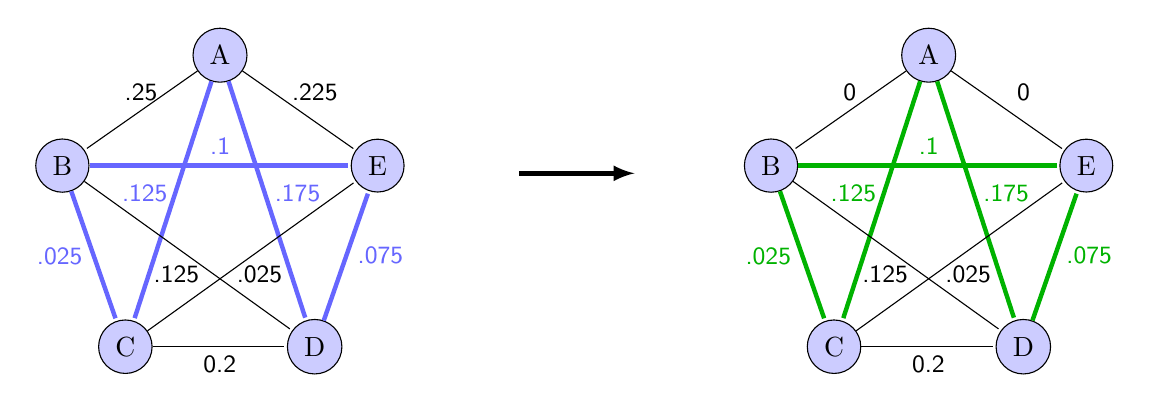
\begin{tikzpicture}[-,shorten >=1pt,auto,node distance=1.7cm,main node/.style={circle, draw, fill=blue!20}]
			% Nodes
			\node [main node] (1) at (0,0) {A};
			\node[main node] (2) [below left of=1, xshift = -0.8cm, yshift = -0.2cm] {B};
			\node[main node] (3) [below of=2, xshift= 0.8cm, yshift = -0.6cm] {C};
			\node[main node] (5) [below right of=1, xshift = 0.8cm, yshift = -0.2cm] {E};
			\node[main node] (4) [below of=5, xshift= -0.8cm, yshift = -0.6cm] {D};
			
			
			
			\path[every node/.style={font=\sffamily\small}]
			(1)
			edge[blue!60,ultra thick] node [right, yshift = 0.1cm, xshift = -0.05cm] {.175} (4)
			edge node[above] {.25} (2)
			edge[blue!60,ultra thick] node[left, yshift = 0.1cm, xshift = 0.08cm] {.125} (3)
			edge node[above, xshift = 0.2cm] {.225} (5)
			
			(2) 
			edge node[below, xshift = -0.15cm] {.125} (4)
			edge[blue!60,ultra thick] node[left] {.025} (3)
			edge[blue!60,ultra thick] node[above] {.1} (5)
			
			(3)
			edge node[below] {0.2} (4)
			edge node[below, xshift = 0.1cm] {.025} (5)
			
			(4) edge[blue!60,ultra thick]  node[right] {.075} (5);
			
			
			
			\node [main node] (6) at (9,0) {A};
			\node[main node] (7) [below left of=6, xshift = -0.8cm, yshift = -0.2cm] {B};
			\node[main node] (8) [below of=7, xshift= 0.8cm, yshift = -0.6cm] {C};
			\node[main node] (10) [below right of=6, xshift = 0.8cm, yshift = -0.2cm] {E};
			\node[main node] (9) [below of=10, xshift= -0.8cm, yshift = -0.6cm] {D};
			
			
			
			\path[every node/.style={font=\sffamily\small}]
			(6)
			edge[black!30!green, ultra thick] node [right, yshift = 0.1cm, xshift = -0.05cm] {.175} (9)
			edge node[above] {0} (7)
			edge[black!30!green, ultra thick] node[left, yshift = 0.1cm, xshift = 0.08cm] {.125} (8)
			edge node[above, xshift = 0.2cm] {0} (10)
			
			(7) 
			edge node[below, xshift = -0.15cm] {.125} (9)
			edge[black!30!green, ultra thick] node[left] {.025} (8)
			edge[black!30!green, ultra thick] node[above] {.1} (10)
			
			(8)
			edge node[below] {0.2} (9)
			edge node[below, xshift = 0.1cm] {.025} (10)
			
			(9) edge[black!30!green, ultra thick] node[right] {.075} (10);
			
			\draw[->, ultra thick, >=latex] (3.8, -1.5) -- (5.3, -1.5);
			
		\end{tikzpicture}
	\end{center}
	
	
	Cycle 9: $A \rightarrow C \rightarrow D \rightarrow B \rightarrow E \rightarrow A$.\;\;\;\;\;\;\;\;\;\;\;\;\;\; $ u_{1830} =  e^{i2\pi(0.775)}$, \;\;\;\;\; $ u'_{1830} =  e^{i2\pi(0.55)}$
	
		\begin{center}	
		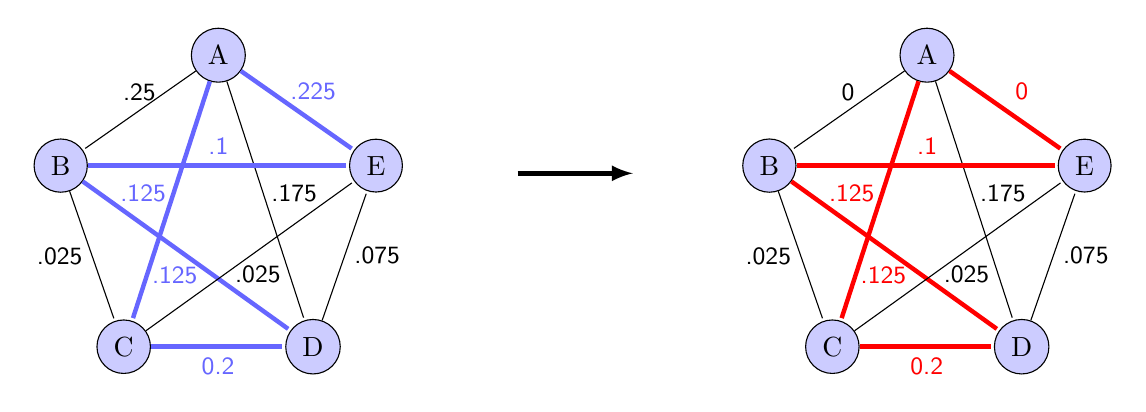
\begin{tikzpicture}[-,shorten >=1pt,auto,node distance=1.7cm,main node/.style={circle, draw, fill=blue!20}]
			% Nodes
			\node [main node] (1) at (0,0) {A};
			\node[main node] (2) [below left of=1, xshift = -0.8cm, yshift = -0.2cm] {B};
			\node[main node] (3) [below of=2, xshift= 0.8cm, yshift = -0.6cm] {C};
			\node[main node] (5) [below right of=1, xshift = 0.8cm, yshift = -0.2cm] {E};
			\node[main node] (4) [below of=5, xshift= -0.8cm, yshift = -0.6cm] {D};
			
			
			
			\path[every node/.style={font=\sffamily\small}]
			(1)
			edge node [right, yshift = 0.1cm, xshift = -0.05cm] {.175} (4)
			edge node[above] {.25} (2)
			edge[blue!60,ultra thick] node[left, yshift = 0.1cm, xshift = 0.08cm] {.125} (3)
			edge[blue!60,ultra thick] node[above, xshift = 0.2cm] {.225} (5)
			
			(2) 
			edge[blue!60,ultra thick] node[below, xshift = -0.15cm] {.125} (4)
			edge node[left] {.025} (3)
			edge[blue!60,ultra thick] node[above] {.1} (5)
			
			(3)
			edge[blue!60,ultra thick] node[below] {0.2} (4)
			edge node[below, xshift = 0.1cm] {.025} (5)
			
			(4) edge node[right] {.075} (5);
			
			\node [main node] (6) at (9,0) {A};
			\node[main node] (7) [below left of=6, xshift = -0.8cm, yshift = -0.2cm] {B};
			\node[main node] (8) [below of=7, xshift= 0.8cm, yshift = -0.6cm] {C};
			\node[main node] (10) [below right of=6, xshift = 0.8cm, yshift = -0.2cm] {E};
			\node[main node] (9) [below of=10, xshift= -0.8cm, yshift = -0.6cm] {D};
			

			\path[every node/.style={font=\sffamily\small}]
			(6)
			edge node [right, yshift = 0.1cm, xshift = -0.05cm] {.175} (9)
			edge node[above] {0} (7)
			edge[red,ultra thick] node[left, yshift = 0.1cm, xshift = 0.08cm] {.125} (8)
			edge [red,ultra thick]node[above, xshift = 0.2cm] {0} (10)
			
			(7) 
			edge [red,ultra thick]node[below, xshift = -0.15cm] {.125} (9)
			edge node[left] {.025} (8)
			edge[red,ultra thick] node[above] {.1} (10)
			
			(8)
			edge [red,ultra thick]node[below] {0.2} (9)
			edge node[below, xshift = 0.1cm] {.025} (10)
			
			(9) edge node[right] {.075} (10);
			
			\draw[->, ultra thick, >=latex] (3.8, -1.5) -- (5.3, -1.5);
			
		\end{tikzpicture}
	\end{center}
	
		Cycle 10: $A \rightarrow C \rightarrow E \rightarrow B \rightarrow D \rightarrow A$.\;\;\;\;\;\;\;\;\;\;\;\;\;\; $ u_{1726} =  e^{i2\pi(0.55)}$, \;\;\;\;\; $ u'_{1726} = e^{i2\pi(0.55)}$
	
	\begin{center}	
		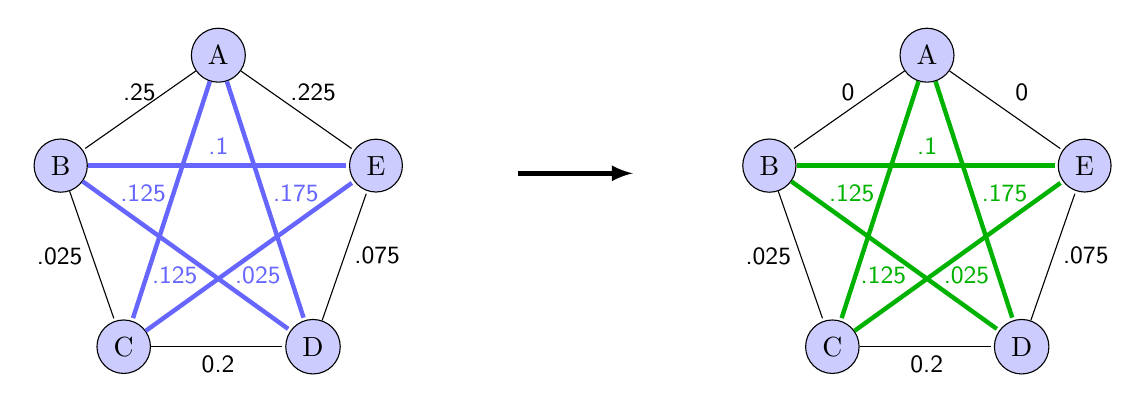
\begin{tikzpicture}[-,shorten >=1pt,auto,node distance=1.7cm,main node/.style={circle, draw, fill=blue!20}]
			% Nodes
			\node [main node] (1) at (0,0) {A};
			\node[main node] (2) [below left of=1, xshift = -0.8cm, yshift = -0.2cm] {B};
			\node[main node] (3) [below of=2, xshift= 0.8cm, yshift = -0.6cm] {C};
			\node[main node] (5) [below right of=1, xshift = 0.8cm, yshift = -0.2cm] {E};
			\node[main node] (4) [below of=5, xshift= -0.8cm, yshift = -0.6cm] {D};
			
			
			
			\path[every node/.style={font=\sffamily\small}]
			(1)
			edge[blue!60,ultra thick] node [right, yshift = 0.1cm, xshift = -0.05cm] {.175} (4)
			edge node[above] {.25} (2)
			edge[blue!60,ultra thick] node[left, yshift = 0.1cm, xshift = 0.08cm] {.125} (3)
			edge node[above, xshift = 0.2cm] {.225} (5)
			
			(2) 
			edge[blue!60,ultra thick] node[below, xshift = -0.15cm] {.125} (4)
			edge node[left] {.025} (3)
			edge[blue!60,ultra thick] node[above] {.1} (5)
			
			(3)
			edge node[below] {0.2} (4)
			edge[blue!60,ultra thick] node[below, xshift = 0.1cm] {.025} (5)
			
			(4) edge node[right] {.075} (5);
			
			\node [main node] (6) at (9,0) {A};
			\node[main node] (7) [below left of=6, xshift = -0.8cm, yshift = -0.2cm] {B};
			\node[main node] (8) [below of=7, xshift= 0.8cm, yshift = -0.6cm] {C};
			\node[main node] (10) [below right of=6, xshift = 0.8cm, yshift = -0.2cm] {E};
			\node[main node] (9) [below of=10, xshift= -0.8cm, yshift = -0.6cm] {D};
			
			
			\path[every node/.style={font=\sffamily\small}]
			(6)
			edge [black!30!green, ultra thick]node [right, yshift = 0.1cm, xshift = -0.05cm] {.175} (9)
			edge node[above] {0} (7)
			edge[black!30!green, ultra thick] node[left, yshift = 0.1cm, xshift = 0.08cm] {.125} (8)
			edge node[above, xshift = 0.2cm] {0} (10)
			
			(7) 
			edge[black!30!green, ultra thick] node[below, xshift = -0.15cm] {.125} (9)
			edge node[left] {.025} (8)
			edge[black!30!green, ultra thick] node[above] {.1} (10)
			
			(8)
			edge node[below] {0.2} (9)
			edge[black!30!green, ultra thick] node[below, xshift = 0.1cm] {.025} (10)
			
			(9) edge node[right] {.075} (10);
			
			\draw[->, ultra thick, >=latex] (3.8, -1.5) -- (5.3, -1.5);
			
		\end{tikzpicture}
	\end{center}

	
		Cycle 11: $A \rightarrow D \rightarrow B \rightarrow C \rightarrow E \rightarrow A$.\;\;\;\;\;\;\;\;\;\;\;\;\;\; $ u_{2230} =  e^{i2\pi(0.575)}$, \;\;\;\;\; $ u'_{2230} = e^{i2\pi(0.35)}$
	
	\begin{center}	
		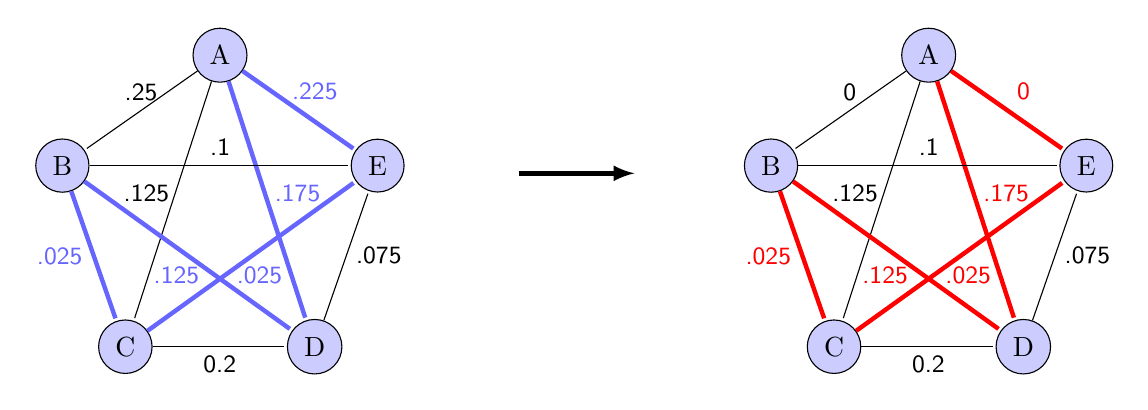
\begin{tikzpicture}[-,shorten >=1pt,auto,node distance=1.7cm,main node/.style={circle, draw, fill=blue!20}]
			% Nodes
			\node [main node] (1) at (0,0) {A};
			\node[main node] (2) [below left of=1, xshift = -0.8cm, yshift = -0.2cm] {B};
			\node[main node] (3) [below of=2, xshift= 0.8cm, yshift = -0.6cm] {C};
			\node[main node] (5) [below right of=1, xshift = 0.8cm, yshift = -0.2cm] {E};
			\node[main node] (4) [below of=5, xshift= -0.8cm, yshift = -0.6cm] {D};
			
			
			
			\path[every node/.style={font=\sffamily\small}]
			(1)
			edge[blue!60,ultra thick] node [right, yshift = 0.1cm, xshift = -0.05cm] {.175} (4)
			edge node[above] {.25} (2)
			edge node[left, yshift = 0.1cm, xshift = 0.08cm] {.125} (3)
			edge[blue!60,ultra thick] node[above, xshift = 0.2cm] {.225} (5)
			
			(2) 
			edge[blue!60,ultra thick] node[below, xshift = -0.15cm] {.125} (4)
			edge[blue!60,ultra thick] node[left] {.025} (3)
			edge node[above] {.1} (5)
			
			(3)
			edge node[below] {0.2} (4)
			edge[blue!60,ultra thick] node[below, xshift = 0.1cm] {.025} (5)
			
			(4) edge node[right] {.075} (5);
			
			\node [main node] (6) at (9,0) {A};
			\node[main node] (7) [below left of=6, xshift = -0.8cm, yshift = -0.2cm] {B};
			\node[main node] (8) [below of=7, xshift= 0.8cm, yshift = -0.6cm] {C};
			\node[main node] (10) [below right of=6, xshift = 0.8cm, yshift = -0.2cm] {E};
			\node[main node] (9) [below of=10, xshift= -0.8cm, yshift = -0.6cm] {D};
			
			
			\path[every node/.style={font=\sffamily\small}]
			(6)
			edge[red,ultra thick] node [right, yshift = 0.1cm, xshift = -0.05cm] {.175} (9)
			edge node[above] {0} (7)
			edge node[left, yshift = 0.1cm, xshift = 0.08cm] {.125} (8)
			edge [red,ultra thick]node[above, xshift = 0.2cm] {0} (10)
			
			(7) 
			edge[red,ultra thick] node[below, xshift = -0.15cm] {.125} (9)
			edge [red,ultra thick]node[left] {.025} (8)
			edge node[above] {.1} (10)
			
			(8)
			edge node[below] {0.2} (9)
			edge [red,ultra thick]node[below, xshift = 0.1cm] {.025} (10)
			
			(9) edge node[right] {.075} (10);
			
			\draw[->, ultra thick, >=latex] (3.8, -1.5) -- (5.3, -1.5);
			
		\end{tikzpicture}
	\end{center}
	
		Cycle 12: $A \rightarrow D \rightarrow C \rightarrow B \rightarrow E \rightarrow A$.\;\;\;\;\;\;\;\;\;\;\;\;\;\; $ u_{2410}  = e^{i2\pi(0.725)}$, \;\;\;\;\; $ u'_{2410}  = e^{i2\pi(0.5)}$
	
	\begin{center}	
		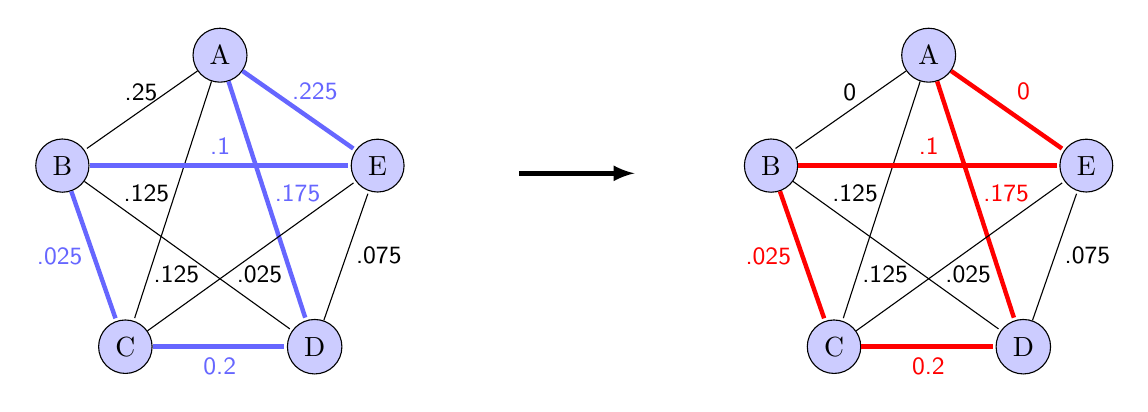
\begin{tikzpicture}[-,shorten >=1pt,auto,node distance=1.7cm,main node/.style={circle, draw, fill=blue!20}]
			% Nodes
			\node [main node] (1) at (0,0) {A};
			\node[main node] (2) [below left of=1, xshift = -0.8cm, yshift = -0.2cm] {B};
			\node[main node] (3) [below of=2, xshift= 0.8cm, yshift = -0.6cm] {C};
			\node[main node] (5) [below right of=1, xshift = 0.8cm, yshift = -0.2cm] {E};
			\node[main node] (4) [below of=5, xshift= -0.8cm, yshift = -0.6cm] {D};
			
			
			
			\path[every node/.style={font=\sffamily\small}]
			(1)
			edge [blue!60,ultra thick]node [right, yshift = 0.1cm, xshift = -0.05cm] {.175} (4)
			edge node[above] {.25} (2)
			edge node[left, yshift = 0.1cm, xshift = 0.08cm] {.125} (3)
			edge [blue!60,ultra thick]node[above, xshift = 0.2cm] {.225} (5)
			
			(2) 
			edge node[below, xshift = -0.15cm] {.125} (4)
			edge[blue!60,ultra thick] node[left] {.025} (3)
			edge [blue!60,ultra thick]node[above] {.1} (5)
			
			(3)
			edge [blue!60,ultra thick]node[below] {0.2} (4)
			edge node[below, xshift = 0.1cm] {.025} (5)
			
			(4) edge node[right] {.075} (5);
			
			\node [main node] (6) at (9,0) {A};
			\node[main node] (7) [below left of=6, xshift = -0.8cm, yshift = -0.2cm] {B};
			\node[main node] (8) [below of=7, xshift= 0.8cm, yshift = -0.6cm] {C};
			\node[main node] (10) [below right of=6, xshift = 0.8cm, yshift = -0.2cm] {E};
			\node[main node] (9) [below of=10, xshift= -0.8cm, yshift = -0.6cm] {D};
			
			
			\path[every node/.style={font=\sffamily\small}]
			(6)
			edge[red,ultra thick] node [right, yshift = 0.1cm, xshift = -0.05cm] {.175} (9)
			edge node[above] {0} (7)
			edge node[left, yshift = 0.1cm, xshift = 0.08cm] {.125} (8)
			edge[red,ultra thick] node[above, xshift = 0.2cm] {0} (10)
			
			(7) 
			edge node[below, xshift = -0.15cm] {.125} (9)
			edge [red,ultra thick]node[left] {.025} (8)
			edge [red,ultra thick]node[above] {.1} (10)
			
			(8)
			edge [red,ultra thick]node[below] {0.2} (9)
			edge node[below, xshift = 0.1cm] {.025} (10)
			
			(9) edge node[right] {.075} (10);
			
			\draw[->, ultra thick, >=latex] (3.8, -1.5) -- (5.3, -1.5);
			
		\end{tikzpicture}
	\end{center}
	
		\subsection{Results: Simulations with Qiskit}  \label{5-city-sim}
	
	Fig. \ref{fig:5-city-circuit} illustrates the circuit for our first Hamiltonian cycle initialized in the eigenstate$|970\rangle  = |001111001010\rangle$. Similar circuits will be executed for the other eleven Hamiltonian cycles, with the only variation being the eigenstate initialization. Our simulations are ideal, implying that our results are not affected by noise. Each circuit is executed 1024 times by default, providing us with a quasi-probability distribution.
	
	\begin{figure}[!h]
		\centering
		\includegraphics[trim={8.5cm 4.4cm 6cm 4.4cm},clip, width=1 \linewidth]{"graphics/5-city-1-cycle-constrained-barrier"}
		\caption{ The quantum circuit for the 5-city graph involves a 3-qubit phase estimation, measuring the Hamiltonian cycle $A \rightarrow B \rightarrow C \rightarrow D \rightarrow E \rightarrow A$. The corresponding eigenstate is $|970\rangle  = |001111001010\rangle$, but due to Qiskit's convention on qubit ordering, the eigenstate is initialized in reverse. The CU gate represents the control unitary matrix containing all the Hamiltonian cycles. The CU' gate includes the same cycles, but before its construction, all edge weights not satisfying the condition ($< 9$) were set to zero. We have two sets of 3 qubits to be measured and stored in classical registers labelled 'output' and 'output c'.
		}
		\label{fig:5-city-circuit}
	\end{figure}
	
	As we did for the 4-city graph, for each Hamiltonian cycle, we can examine the two states with the highest counts and summarize them in Table \ref{table:sim-results-5-city}. This table also presents 4-qubit estimation.
	
		\begin{figure}[!h]
		\centering
		\includegraphics[width=\textwidth,height=0.9\textheight,keepaspectratio]{"graphics/1-3-5city"}
		\caption{3 qubit (left column) \& 4 qubit (right column) phase estimation for the 5-city graph. Hamiltonian cycles: 1 to 3}
		\label{fig:5-city-1-3}
	\end{figure}		
	
	\begin{figure}[!h]
		\centering
		\includegraphics[ width=\textwidth,height=0.9\textheight,keepaspectratio]{"graphics/4-6-5city"}
		\caption{3 qubit (left column) \& 4 qubit (right column) phase estimation for the 5-city graph. Hamiltonian cycles: 4 to 6}
		\label{fig:5-city-4-6}
	\end{figure}		
	
	\begin{figure}[!h]
		\centering
		\includegraphics[width=\textwidth,height=0.9\textheight,keepaspectratio]{"graphics/7-9-5city"}
		\caption{3 qubit (left column) \& 4 qubit (right column) phase estimation for the 5-city graph. Hamiltonian cycles: 7 to 9}
		\label{fig:5-city-7-9}
	\end{figure}		
	
	\begin{figure}[!h]
		\centering
		\includegraphics[width=\textwidth,height=0.9\textheight,keepaspectratio]{"graphics/10-12-5city"}
		\caption{3 qubit (left column) \& 4 qubit (right column) phase estimation for the 5-city graph. Hamiltonian cycles: 10 to 12}
		\label{fig:5-city-10-12}
	\end{figure}		
	
	\begin{table}[ht!]
		\centering
		\begin{tabular}{lllllll} 
			\toprule
					Cycle & Expected & Phase Qubits & Highest Counts & Prob. & 2nd Highest Counts & Prob. \\
			\midrule
			\multirow{2}{*}{1} & \multirow{2}{*}{$0.3, \; 0.775$} & 3 & $0.25, \; 0.75$ & $52\%$ &  $0.375, \; 0.75$  & $23\%$ \\
			&                          & 4& $0.3125, \; 0.75$ & $50\%$ &  $0.3125, \; 0.8125$  & $21\%$ \\
			\hline
			\multirow{2}{*}{2} & \multirow{2}{*}{$0.3, \; 0.55$} & 3 & $0.25, \; 0.5$ & $35\%$ &  $0.25, \; 0.625$  & $14\%$ \\
			&                          & 4& $0.3125, \; 0.5625$ & $75\%$ &  $0.3125, \; 0.5$  & $6\%$ \\
			\hline
			\multirow{2}{*}{3} & \multirow{2}{*}{$0.35, \; 0.825$ } & 3 & $0.375, \; 0.875$ & $50\%$ &  $0.375, \; 0.75$  & $24\%$ \\
			&                          & 4& $0.375, \; 0.8125$ & $47\%$ &  $0.3125, \; 0.8125$  & $23\%$ \\
			\hline
			\multirow{2}{*}{4} & \multirow{2}{*}{$0.35, \; 0.6$} & 3 & $0.375, \; 0.625$ & $78\%$ &  $0.25, \; 0.625$  & $5\%$ \\
			&                          & 4& $0.375, \; 0.625$ & $31\%$ &  $0.3125, \; 0.625$  & $16\%$ \\
			\hline
			\multirow{2}{*}{5} & \multirow{2}{*}{$0.5, \; 0.75$} & 3 & $0.5, \; 0.75$ & $100\%$ & & \\
			&                          & 4& $0.5, \; 0.75$ & $100\%$ &   &  \\
			\hline
			\multirow{2}{*}{6} & \multirow{2}{*}{$0.5, \; 0.75$} & 3 & $0.5, \; 0.75$ & $100\%$ & & \\
			&                          & 4& $0.5, \; 0.75$ & $100\%$ &   &  \\
			\hline
			\multirow{2}{*}{7} & \multirow{2}{*}{$0.35, \; 0.575$ } & 3 & $0.375, \; 0.625$ & $51\%$ &  $0.375, \; 0.5$  & $23\%$ \\
			&                          & 4& $0.375, \; 0.5625$ & $50\%$ &  $0.3125, \; 0.5625$  & $21\%$ \\
			\hline
			\multirow{2}{*}{8} & \multirow{2}{*}{$0.5, \; 0.5$} & 3 & $0.5, \; 0.5$ & $100\%$ &   &  \\
			&                          & 4& $0.5, \; 0.5$ & $100\%$ &   &  \\
			\hline
			\multirow{2}{*}{9} & \multirow{2}{*}{$0.55, \; 0.775$} & 3 & $0.5, \; 0.75$ & $52\%$ &  $0.625, \; 0.75$  & $22\%$ \\
			&                          & 4& $0.5625, \; 0.75$ & $51\%$ &  $0.5625, \; 0.8125$  & $22\%$ \\
			\hline
			\multirow{2}{*}{10} & \multirow{2}{*}{$0.55, \; 0.55$ } & 3 & $0.5, \; 0.5$ & $32\%$ &  $0.5, \; 0.625$  & $17\%$ \\
			&                          & 4& $0.5625, \; 0.5625$ & $75\%$ &  $0.5625, \; 0.5$  & $5\%$ \\
			\hline
			\multirow{2}{*}{11} & \multirow{2}{*}{$0.35, \; 0.575$} & 3 & $0.375, \; 0.625$ & $49\%$ &  $0.375, \; 0.5$  & $22\%$ \\
			&                          & 4& $0.375, \; 0.5625$ & $51\%$ &  $0.3125, \; 0.5625$  & $20\%$ \\
			\hline
			\multirow{2}{*}{12} & \multirow{2}{*}{$0.50, \; 0.725$ } & 3 & $0.5, \; 0.75$ & $88\%$ &  $0.5, \; 0.625$  & $5\%$ \\
			&                          & 4& $0.5, \; 0.75$ & $58\%$ &  $0.5, \; 0.6875$  & $24\%$ \\
			
			\bottomrule
		\end{tabular}
		\caption{Simulation results for the 5-city graph.}
		\label{table:sim-results-5-city}
	\end{table} 
	
	
 	
	
	
	\chapter{Discussion}
	
Referring to Table \ref{table:sim-results-4-city}, we observe that cycle 1 represents the solution for our 4-city problem, as our expected phase estimation before and after satisfying the condition is both equal to $0.85$. With 3-qubit estimation, we achieved a $77\%$ quasi-probability of measuring the state $0.875, 0.875$. This suggests that the most probable result indicates the cycle as a solution. One might expect a better quasi-probability as we increase the number of phase qubits, as it should provide a finer estimate of our phases. However, with 4-qubit estimation, our quasi-probability for the most measured state, $0.875, 0.875$, drops to $34\%$. Despite this decrease, it remains the state with the most counts, indicating equality of our two phases and thus a solution. Further, 5-qubit estimation restores the quasi-probability for the most measured state, in this case, $0.84375, 0.84375$, to $77\%$. This suggests that increasing the number of phase qubits does not necessarily increase the probability of measuring a single state. To further elaborate on why this is the case, we can examine the representation of $0.85$ in binary:
	
	$$0.11011001100110011...$$
	
Since the binary representation of $0.85$ is recurring, perfect accuracy with phase estimation is unattainable. This same challenge arises in our 5-city simulation, where cycle 10 (Fig. \ref{fig:5-city-10-12}) represents our solution, and the phase we aim to estimate is $0.55$, which also recurs in binary. In both cases, we can only establish a very good approximate value. To illustrate this further, let's examine the resolution of 3, 4, and 5 qubit estimation below and refer to Fig. \ref{fig:phase-precision} to understand the probabilities.
	
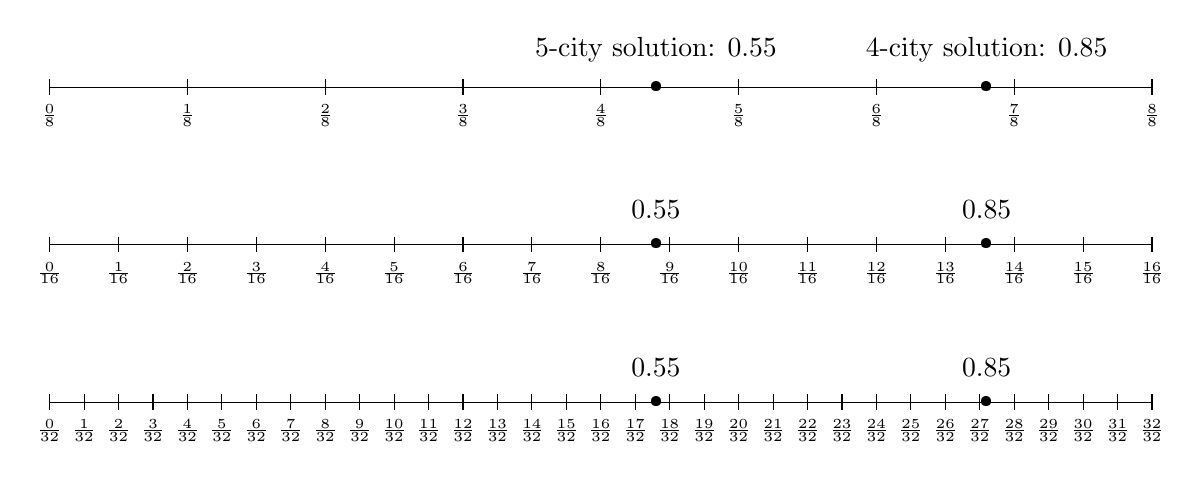
\begin{tikzpicture}
	\pgfmathsetmacro{\lineLength}{14}
	
	% First line - 1/8 steps
	\node[label=above:{5-city solution: 0.55}] at (0.55*\lineLength,0) {\textbullet};
	\node[label=above:{4-city solution: 0.85}] at (0.85*\lineLength,0) {\textbullet};
	\draw (0,0) -- (\lineLength,0);
	\foreach \x in {0,1,...,8} { 
		\draw (\x/8*\lineLength ,0.1) -- (\x/8*\lineLength ,-0.1) node[below] {\tiny$\frac{\x}{8}$};
	}
	
	% Second line - 1/16 steps
	\node[label=above:{0.55}] at (0.55*\lineLength,-2) {\textbullet};
	\node[label=above:{0.85}] at (0.85*\lineLength,-2) {\textbullet};
	\draw (0,-2) -- (\lineLength,-2);
	\foreach \x in {0,1,...,16} { 
		\draw (\x/16*\lineLength,-1.9) -- (\x/16*\lineLength,-2.1) node[below] {\tiny$\frac{\x}{16}$};
	}
	
	% Third line - 1/32 steps
	\node[label=above:{0.55}] at (0.55*\lineLength,-4) {\textbullet};
	\node[label=above:{0.85}] at (0.85*\lineLength,-4) {\textbullet};
	\draw (0,-4) -- (\lineLength,-4);
	\foreach \x in {0,1,...,32} {
		\draw (\x/32*\lineLength,-3.9) -- (\x/32*\lineLength,-4.1) node[below] {\tiny$\frac{\x}{32}$};
	}
	
\end{tikzpicture}
	
An intuitive way to interpret the number lines is that when the value is near a specific step, that step becomes more likely to be measured. If the value falls perfectly between two steps, the best possible approximation is either the lower or upper bound, both with an equal probability, approximately $P_b \approx 40\%$. It's important to note that we are measuring two independent phases for each Hamiltonian cycle, so our best approximation will be $P_b^2 \approx 16\%$.
	
We can see for the 4-qubit estimation, the introduction of a more precise value of $13/16$ increased its probability of being measured as a good approximation for $0.85$, and in turn decreased the probability of $7/8 = 14/16$ being measured. Performing 5-qubit estimation does improve our results but does not justify the computational cost considering we achieved similar results with 3-qubit estimation. We see a similar issue with our results for the 5-city problem; we only simulated 3 and 4-qubit estimation, but had we done 5, our confidence in the result would have decreased.
	
Unless we obtain a fortunate solution as in cycle 8 of the 5-city problem (Fig. \ref{fig:5-city-7-9}), where our $\phi = 0.5$, can be represented exactly, we need to run phase estimation a number of times from which we can use the mode of our results as the solution. And as we've discussed earlier, using a larger number of phase qubits does not necessarily improve your confidence in the result. If we only consider the states with the highest counts in Tables \ref{table:sim-results-4-city} \& \ref{table:sim-results-5-city}, then our results perfectly predict the solutions and non-solutions.
	
The question we need to ask now is how many phase qubits are needed to correctly identify a solution or non-solution based on the most frequent state measured? And the answer is we need to make sure the resolution of our phase qubits to be finer than the condition value, $\alpha$. Let's consider a non-solution where the reduction to $\phi$ is exactly the resolution of 3-qubit estimation, $\alpha = 0.125$:
	
	
	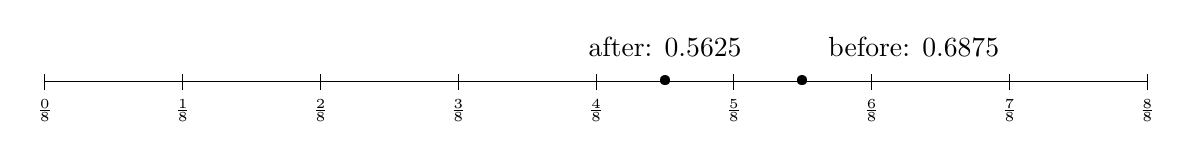
\begin{tikzpicture}
		\pgfmathsetmacro{\lineLength}{14}
		
		% First line - 1/8 steps
		%\node[label=above :{0.5}] at (0.5*\lineLength,0) {\textbullet};
		\node[label=above:{after: 0.5625}] at (0.5625*\lineLength,0) {\textbullet};
		\node[label=above right :{before: 0.6875}] at (0.6875*\lineLength,0) {\textbullet};
		\draw (0,0) -- (\lineLength,0);
		\foreach \x in {0,1,...,8} { 
			\draw (\x/8*\lineLength ,0.1) -- (\x/8*\lineLength ,-0.1) node[below] {\tiny$\frac{\x}{8}$};
		}
	\end{tikzpicture}
	
	
	Based on our best approximation, we are likely to obtain any of the following four results most frequently with $P^2_b \approx 16\%$:

	$$P_1: 0.625, 0.625$$
	$$P_2: 0.500, 0.625$$
	$$P_3: 0.625, 0.750$$
	$$P_4: 0.500, 0.750$$
	
	Here, we run the risk of selecting $P_1$, which implies a solution. By extending the distance between our $\phi$ values, we reduce the probability of measuring $0.625$. We can predict, based on qualitative analysis, how probable our four results above will be:
	
		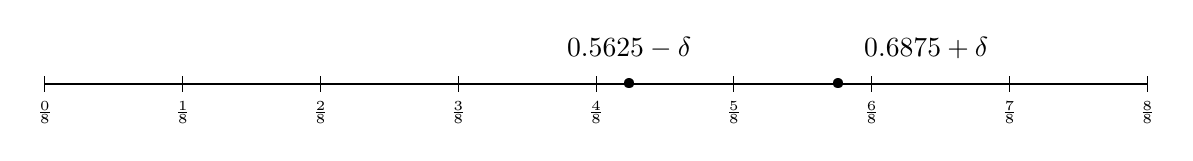
\begin{tikzpicture}
		\pgfmathsetmacro{\lineLength}{14}
		
		\node[label=above:{$0.5625-\delta$}] at (0.53*\lineLength,0) {\textbullet};
		\node[label=above right :{$0.6875 + \delta$}] at (0.72*\lineLength,0) {\textbullet};
		\draw (0,0) -- (\lineLength,0);
		\foreach \x in {0,1,...,8} { 
			\draw (\x/8*\lineLength ,0.1) -- (\x/8*\lineLength ,-0.1) node[below] {\tiny$\frac{\x}{8}$};
		}
	\end{tikzpicture}
	
 $$P_1 < P_2 = P_3 < P_4$$
 
We actually simulated a similar case in cycle 7 of our 5-city problem (Fig. \ref{fig:5-city-7-9}), where the least probable result of the top four states indicated the cycle was a solution. If $\delta << 1$, we would have to run our circuit many times over to appropriately measure the non-solution as the most frequent result. Otherwise, we run the risk again of predicting a solution with $P_1$ as it would be very close to $P_4$. A safe bet would be to have a phase resolution at least twice the condition value. Let's illustrate this again by inconveniently placing the phases we hope to estimate perfectly in between steps:
 
 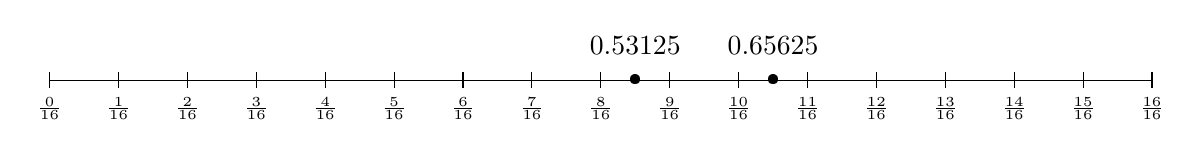
\begin{tikzpicture}
 	\pgfmathsetmacro{\lineLength}{14}
 	
	% Second line - 1/16 steps
\node[label=above:{0.53125}] at (0.53125*\lineLength,-2) {\textbullet};
\node[label=above:{0.65625}] at (0.65625*\lineLength,-2) {\textbullet};
\draw (0,-2) -- (\lineLength,-2);
\foreach \x in {0,1,...,16} { 
	\draw (\x/16*\lineLength,-1.9) -- (\x/16*\lineLength,-2.1) node[below] {\tiny$\frac{\x}{16}$};
}
 \end{tikzpicture}
 
 We now run no risk of the four most probable states indicating a solution. As our measurement will likely collapse to any of these four options with $P^2_b \approx 16\%$:
 
 $$P_1: 0.5000, 0.6250$$
 $$P_2: 0.5000, 0.6875$$
 $$P_3: 0.5625, 0.6250$$
 $$P_4: 0.5625, 0.6875$$
 
We can further demonstrate that in the case of a solution, two of the four states will indicate it as a solution, while the other two will not. However, this discrepancy can be attributed to rounding errors, as our condition would result in a much greater reduction in phase. To illustrate, let's consider the phase $0.65625$:


 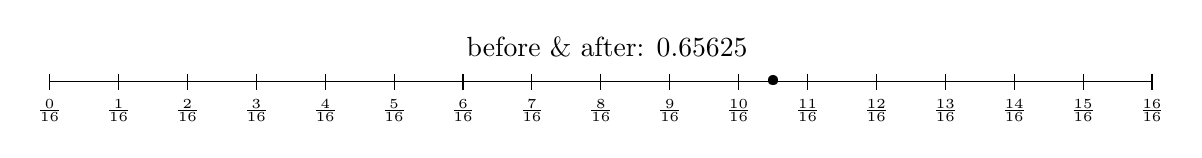
\begin{tikzpicture}
	\pgfmathsetmacro{\lineLength}{14}
	
	% Second line - 1/16 steps
	\node[label=above left :{before \& after: 0.65625}] at (0.65625*\lineLength,-2) {\textbullet};
	\draw (0,-2) -- (\lineLength,-2);
	\foreach \x in {0,1,...,16} { 
		\draw (\x/16*\lineLength,-1.9) -- (\x/16*\lineLength,-2.1) node[below] {\tiny$\frac{\x}{16}$};
	}
\end{tikzpicture}

$$P_1: 0.6250, 0.6250$$
$$P_2: 0.6250, 0.6875$$
$$P_3: 0.6875, 0.6250$$
$$P_4: 0.6875, 0.6875$$


We can also discuss the number of eigenstate qubits needed. Our method asks us to construct a matrix of size $N^N \times N^N$, where $N$ represents the number of cities. This does result in a unitary matrix however, it cannot be neccesarily represented by an exact number of qubits. We encountered this issue in our 5-city graph, where we introduced ones at the end of the matrix, Equation \eqref{ones}. If $n$ represents the number of qubits we need and $m$ represents the number of cities, we need to solve the equation:

$$2^n = m^m$$
$$n = m\mathrm{log}_2(m)$$

We can conclude that the number of eigenstate qubits needed will scale polynomially, where it is less than $m^2$. For example, in the case of 5 cities, $n \approx 11.6$, which we round up to 12 qubits.

Finally, because we iterate through all Hamiltonian cycles to solve this problem, our time complexity remains $O((N-1)!)$. Alternatively, we can solve this decision problem by running all Hamiltonian cycles in parallel, which reduces our execution time. However, the tradeoff would be introducing exponential space complexity, $O((N-1)!)$.
	
	\bibliographystyle{unsrt}

	\bibliography{ref}

	\appendix
	\chapter{Hamiltonian Cycles and Locating Eigenstates Code}
	
	The code detailed in this section can generate the information found in Tables \ref{table:ham-cycle-details-4-city}, \ref{table:4-city-conversions},  \ref{table:ham-cycle-details-5-city} and \ref{table:5-city-conversions}, which construct the Hamiltonian cycles and locate the eigenstates. 
	
	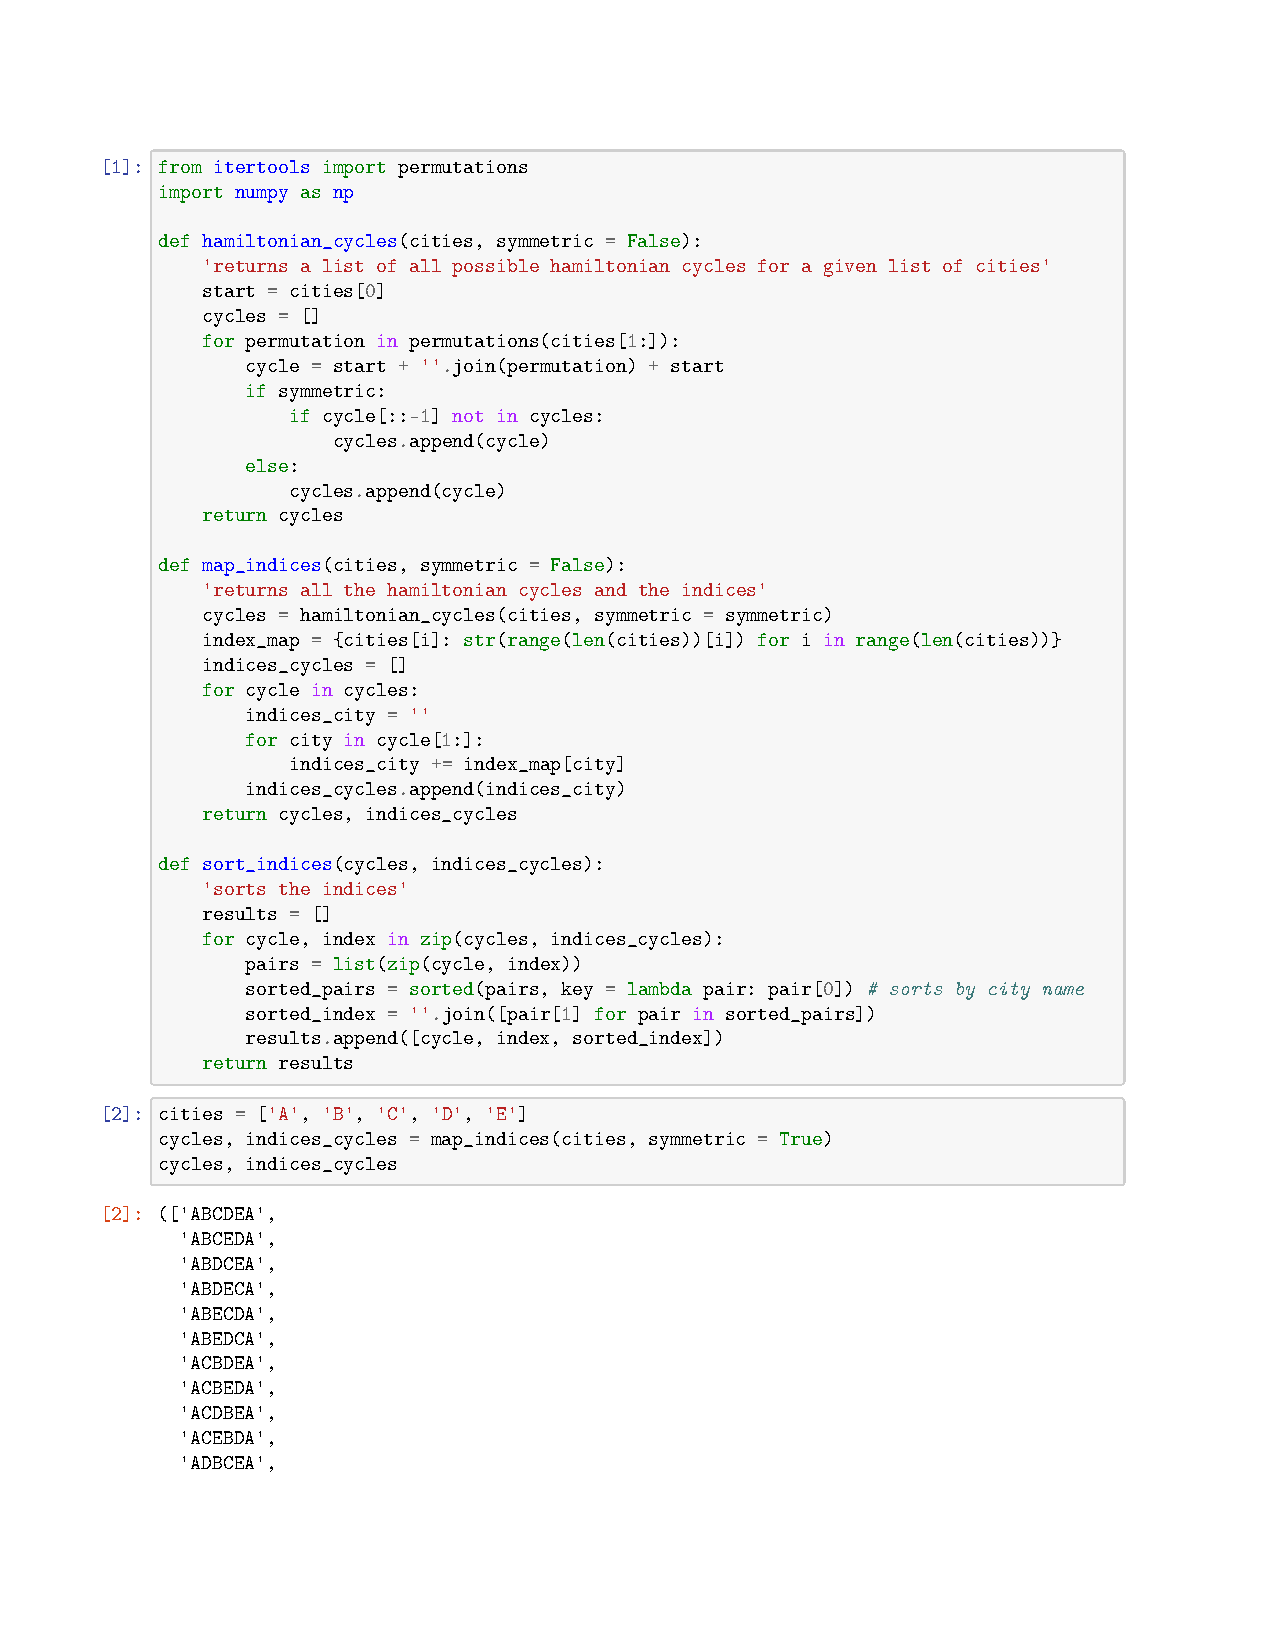
\includepdf[pages=-]{hamiltonian_cycles.pdf}
	\chapter{Simulation Code with Qiskit}
	
	The code detailed in this section demonstrates simulations for the four-city graph, as discussed in Section \ref{4-city-sim}. This code can be extended to model the five-city graph presented in Section \ref{5-city-sim}, and can be further adapted to accommodate even larger city graphs.
	
	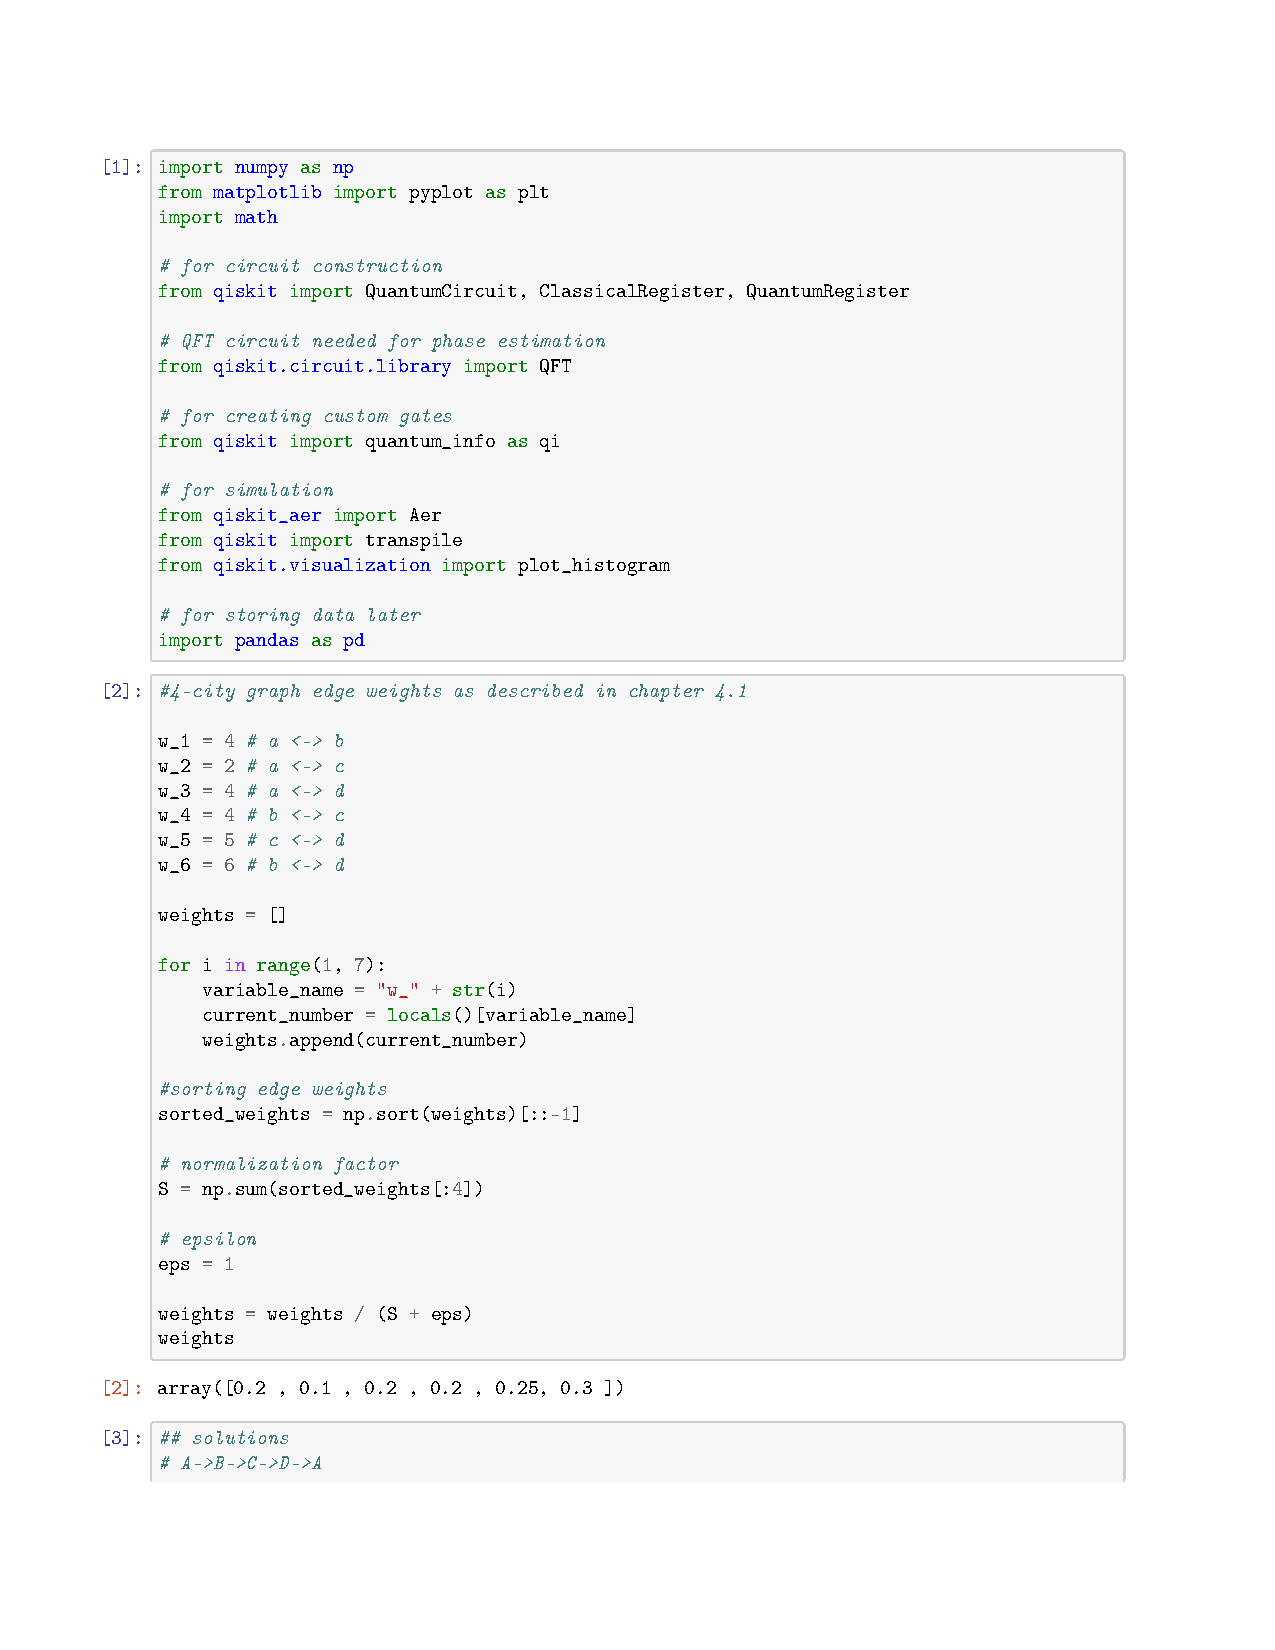
\includepdf[pages=-]{4-city-code/4-city-code.pdf}
	
	\backmatter
	
	
	\end{document}
	
	
	
\end{document}
